\chapter{Results}\label{Chap:Results}
In this section the results from the FLEXPART and FLEXDUST model simulations are presented following the methods described in the previous sections. First the results from the modelsensitivity analysis and model validation are presented in \Cref{sec:sensitvity_experiment} and \Cref{sec:model_eval} respectively. 
In  \Cref{sec:result_average} the average state of emission transport and deposition are examined. For each location the mean dust transport path and main source regions are determined for both the fine clay and coarse silt particle size bins. 
Then in \Cref{sec:inter_annual_results} the inter annual variation in spring dust emissions, transport and deposition over the 20 year period are investigated. The composite analysis of the of the circulation during the preceeding winter in strong and weak deposition years show a strong positive MSLP anomalies over the arctic implying a negative \acrshort{ao}.   

\section{Model sensitivity to input data and parameters}\label{sec:sensitvity_experiment}
Sensitivity experiments are a crucial part of any modelling study. The aim of a sensitivity analysis is to quantify the impact of possible errors in the input data on the predicted model output. 
In \Cref{sec:sens_forcing} the impact of meteorological forcing on the simulated dust emissions and deposition is examined by comparing ERA5 and ERA-Interim forced simulations
. Sand and clay fractions are important input variables in FLEXDUST (\Cref{sec:flexdust}), therefore the sensitivity of simulated dust emission to the choice of soil texture data set is considered in \Cref{sec:sens_soil}. \Cref{sec:density_experiment} and \Cref{wet:dep_sensitivty} the sensitivity of estimated deposition to the choice of particle density and cloud scavenging parameters are investigated. 
\subsection{Sensitivity to forcing data}\label{sec:sens_forcing}

\begin{figure}[htpb]
    \centering
    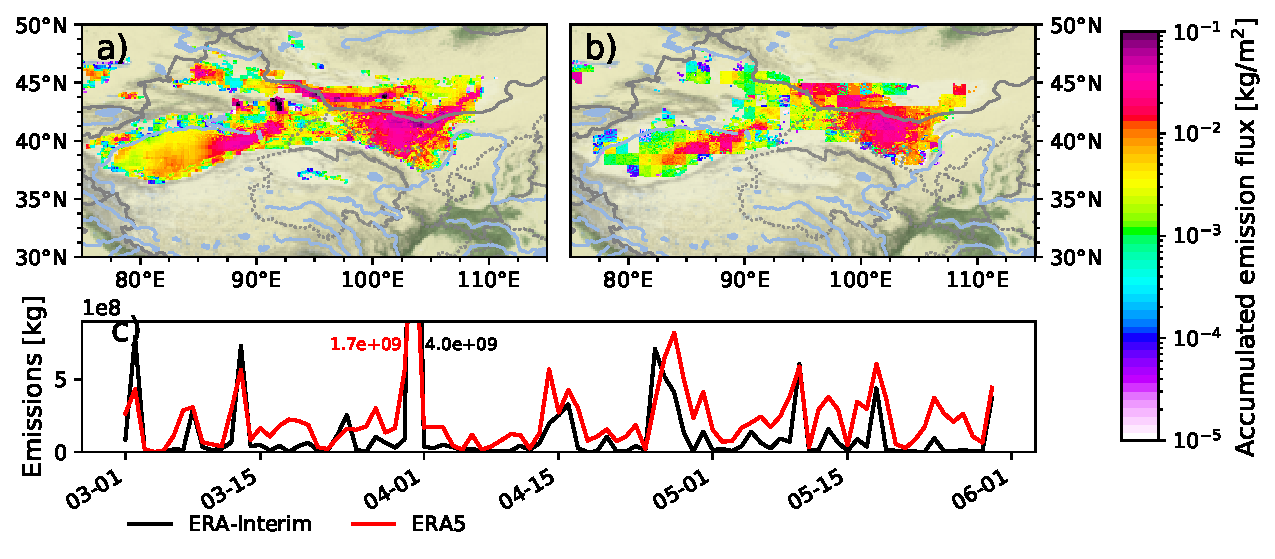
\includegraphics[width=\textwidth]{texfiles/figs/emissions_ERA5_ERA-interim.pdf}
    \caption{Accumulated emission flux  (\si{\kg\per\square\metre}) simulated by FLEXDUST for the spring of 2015. (a) ERA5 0.3\degree resolution and (b) ERA-Interim 1\degree resolution. (c) The time series of daily accumulated emissions ERA-interim (red) and ERA-5 (black) }
    \label{fig:ERA5_ERA-interim_emissions}
\end{figure}
To better understand how errors in meteorological forcing impacts the model results, FLEXPART and FLEXDUST simulations forced by both ERA5 and ERA-Interim was done for the spring of 2015. Compared to ERA-interim, ERA5 features a more recent version of the IFS, higher spatial resolution 0.3\degree compared to 1\degree and increased number of vertical levels. 
\par \Cref{fig:ERA5_ERA-interim_emissions} shows the dust emission flux simulated by FLEXDUST with (a) ERA5 and (b) ERA-Interim. The impact of the coarser resolution of ERA-Interim is noticeable.  The modelled dust emissions over Taklamakan are particularly sensitive to the spatial resolution of the forcing due to the complex topography of the surrounding mountains, that cannot be resolved by coarser resolution of ERA-Interim. Another feature that is missing in the ERA-Interim simulation is the boundary between the Mongolia and the deserts north west of the CLP. There are also major differences in the temporal evolution of simulated dust emissions (\Cref{fig:ERA5_ERA-interim_emissions}c) both in the magnitude and frequency. In the ERA-Interim simulation the most intense dust events show higher dust emissions compared to ERA5, however for the weaker dust events the opposite is true. This suggest that large dust storms, which are usually caused by synoptic scale frontal activity are less sensitive to the resolution of the forcing compared to the weaker dust events.

\begin{figure}[htbp]
    \centering
    \includegraphics[width=\textwidth]{texfiles/figs/era5_era_interim_depo_tranpsort.pdf}
    \caption{Accumulated source contribution and emission sensitivity for ERA5 (a),(b) and ERA-interim (d),(d) for total deposition of coarse silt during the spring of 2015. (e) time series of daily accumulated emission fl{}ux for ERA5 (red) and ERA-Interim (black).}
    \label{fig:era5_era_interim_source}
\end{figure}

Further more the source contribution of total deposition (\Cref{fig:era5_era_interim_source}) show an even higher sensitivity to input forcing. This might be partly because of ERA-Interim forced simulation showing weaker emissions from weak and moderate dust events than the ERA5 forced simulation. 
This also consistent with the largest deposition episode not coinciding with the strong emission events.
\subsection{Sensitivity to soil texture data}\label{sec:sens_soil}
The dust emission scheme used in FLEXDUST assume that the sand blasting efficiency (\Cref{eq:sand_blasing_eff}) increases exponentially with $f_{clay}$ for $f_{clay} \leq 0.2$. Consequently the simulated dust emission might be very sensitive to the soil texture data set used.
During the process of performing these sensitivity experiments it was discovered that original soil texture dataset had a very small clay fraction over the Taklamakan (\Cref{fig:clay_sand_fraction_comparison}a). This resulted in FLEXDUST barely simulating any emissions from Taklamakan.

\begin{figure}[hptb]
    \centering
    \includegraphics[width=\textwidth]{texfiles/figs/clay_sand_fraction.pdf}
    \caption{Clay and sand fraction maps from 3 different data sources: default clay (a), CLM clay (b), ISRIC clay (c), default sand (d), CLM sand (e) and ISRIC sand (f)}
    \label{fig:clay_sand_fraction_comparison}
\end{figure}

To address this bias, new sand and clay maps from the SoilGrids database maintained by ISRIC were implemented in FLEXDUST. The SoilGrids soil maps uses state-of-the-art machine learning methods to map the spatial distribution of soil properties across the globe. Providing a map soil properties at 250 meter spatial resolution. As shown in \Cref{fig:clay_sand_fraction_comparison} ISRIC clay and sand fractions has a higher clay fraction over Taklamakan compared to the default soil maps. The accumulated modelled emissions for 2019 are shown in \Cref{fig:emissions_ISRIC_old_com}, (a) using the default soil maps and (b) with new ISRIC maps. The difference between the two is noticeable, with the new ISRIC maps Taklamakan is now represented as a major dust source.

\begin{figure}[htpb]
    \centering
    \includegraphics[width=\textwidth]{texfiles/figs/emssion_field_old_vs_isric_2019.pdf}
    \caption{Accumulated simulated dust emissions for 2019, default soil maps (a), and ISRIC soil maps (b).}
    \label{fig:emissions_ISRIC_old_com}
\end{figure}
\subsection{Sensitivity to particle density}\label{sec:density_experiment}
The density of mineral dust particles vary depending on the mineralogical composition of the dust particle. To examine how the density of the dust particle affects the long range transport and the amount of deposited material, backwards
FLEXPART simulations with varying particle density from \SI{2200}{\kg\per\cubic\cm} to \SI{2800}{\kg\per\cubic\cm}  were conducted  at the SACOL site for the spring of 2019. 
In \Cref{fig:dry_dep_density} and \Cref{fig:wet_dep_density} the rate of dry and wet deposition are plotted for different densities and a least squares fit is done to the data. The rate of  increase approximately linearly with increasing particle density. The density has a bigger impact on the deposition rate of the coarse particles (\Cref{fig:dry_dep_density}b, \Cref{fig:wet_dep_density}), where the rate of deposition of the heaviest particle is almost twice that of the lightest particle. In comparison to the fine particles which only show about a 2\% difference between the lightest and heaviest particle in the dry deposition rate. The wet deposition is more sensitive to the particle density compared to the dry deposition for both the fine and coarse particles. 
\begin{figure}[hptb]
    \centering
    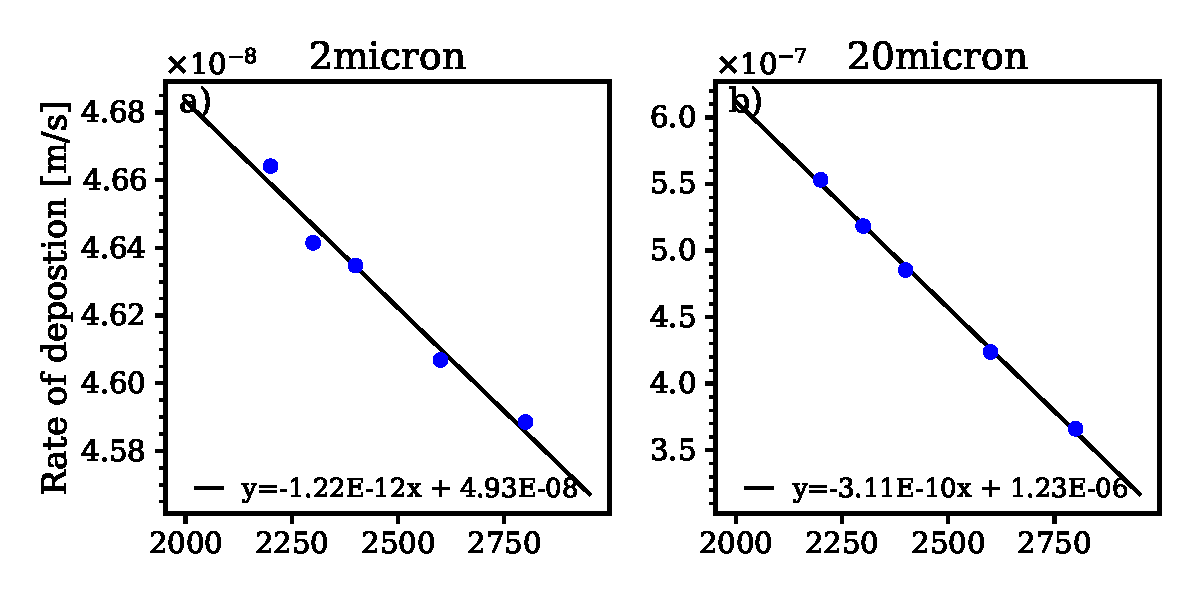
\includegraphics[width=\textwidth]{texfiles/figs/drydep_function_of_density.pdf}
    \caption{Dry deposition rate at the SACOL site as function of dust particle density, (a) Fine clay, (b) coarse silt}
    \label{fig:dry_dep_density}
\end{figure}

\begin{figure}[hptb]
    \centering
    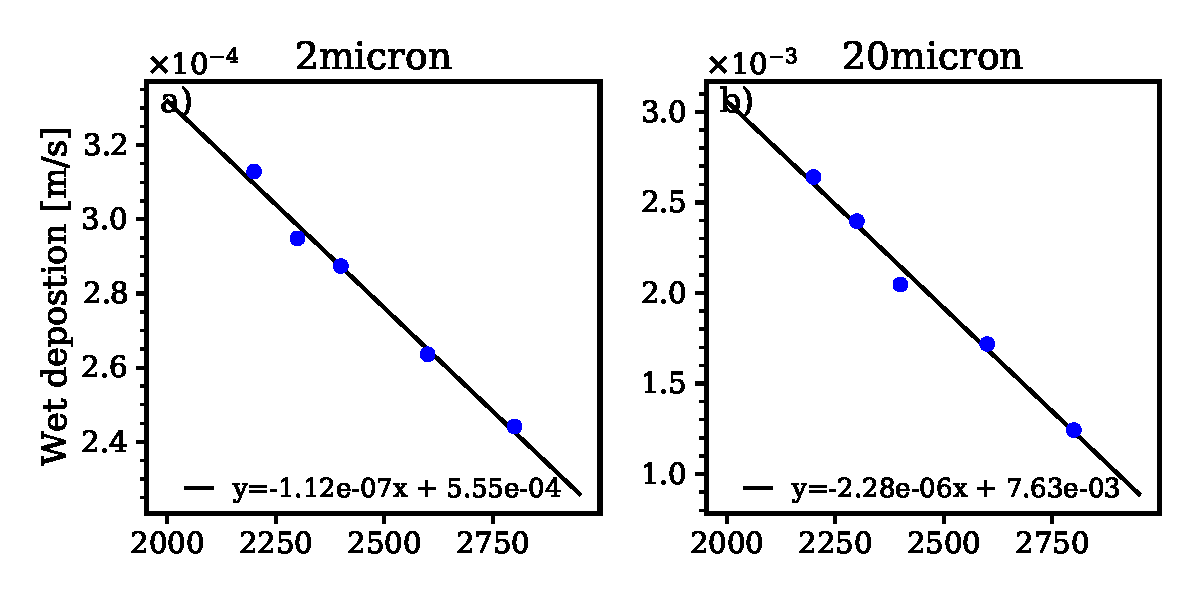
\includegraphics[width=\textwidth]{texfiles/figs/wetdep_function_of_density.pdf}
    \caption{The wet deposition rate at the SACOL site as function of dust particle density, (a) Fine clay, (b) coarse silt}
    \label{fig:wet_dep_density}
\end{figure}

\subsection{Sensitivity to cloud scavenging scheme}\label{wet:dep_sensitivty}
To test how the different model parameters affect the simulated wet deposition. FLEXDUST was run with both with and without the below cloud scavenging turned on. \Cref{fig:scav_sensitivty} shows the difference between having the below cloud scavenging scheme turned on and off. There is a higher contribution from the proximal regions with the below cloud scavenging turned on.  
\begin{figure}[htbp]
    \centering
    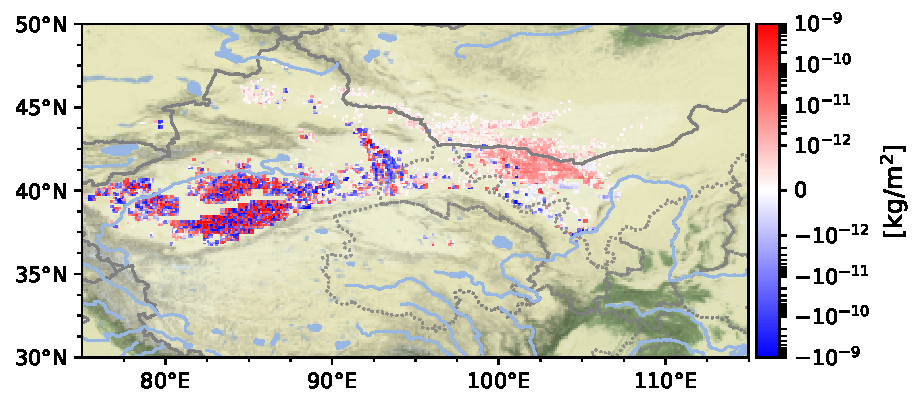
\includegraphics[width=\textwidth]{texfiles/figs/no_scav_test.pdf}
    \caption{The difference in the source contribution to the wet depostion at BADOE. With below cloud scavanging turned on minus below cloud scavanging turned off}
    \label{fig:scav_sensitivty}
\end{figure}

\section{Model evaluation against observation}\label{sec:model_eval}
\begin{figure}
    \centering
    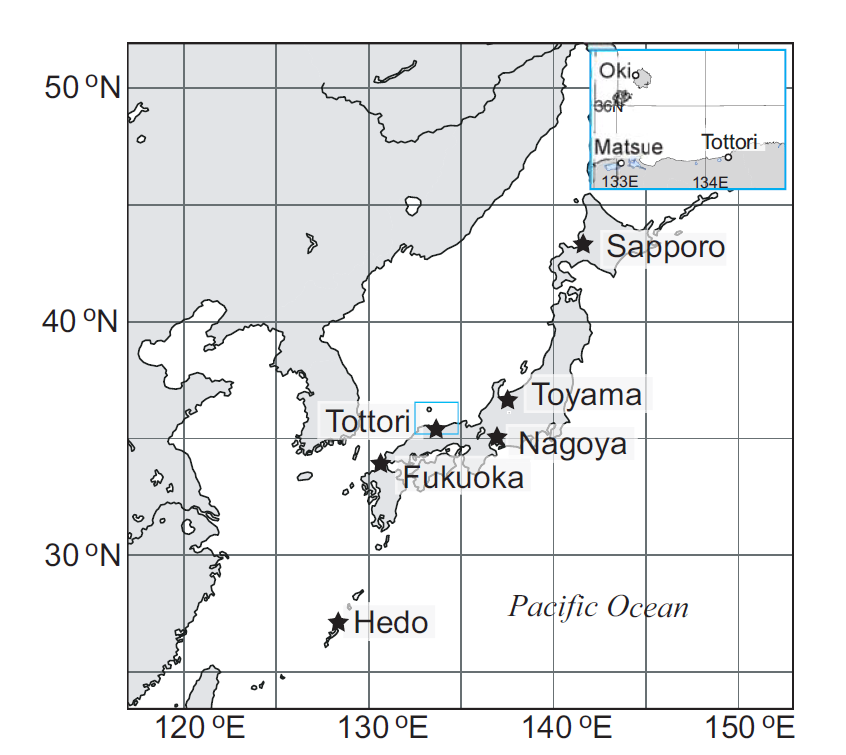
\includegraphics[scale=0.45]{texfiles/figs/Osada_locations.PNG}
    \caption{Map of the locations where dust deposition where sampled \parencite{osada2014wet}}
    \label{fig:map_japan}
\end{figure}
There is a very limited amount of measurements of dust deposition fluxes that both separate dry and wet deposition and has a sufficient temporal resolution to be use for evaluating the performance of FLEXPART/FLEXDUST. \textcite{osada2014wet} published a data set of monthly dry and wet deposition fluxes from 6 locations by the coast of japan providing measurement from November 2008 until December 2010. They used a 4-stage filtration approach to separate the deposited dust into four size bins  >\SI{20}{\micro\metre}, \SI{20}{\micro\metre}-\SI{10}{\micro\metre}, \SI{10}{\micro\metre}-\SI{5}{\micro\metre} and \SI{5}{\micro\metre}-\SI{1}{\micro\metre}. These particles size bins were simulated separately in FLEXPART and then added together in post processing. The backward simulations were conducted for the Hedo, Fukuoka, Tottori and Toyama site to in order to evaluate how well this dust model is able to reproduce the spatial variation. 

\Cref{fig:model_eval_dry_deposition} show the time series of observed and modelled monthly dry deposition fluxes for the 4 locations that where selected. Evident is FLEXPART ability to reproduce the spatial variation between the sites with Tottori and Toyama experiencing the strongest deposition. The inter annual variation between the two years is also reasonable reproduced in the model, with stronger deposition during 2010 compared to 2009 in both the observation and the model. \par \Cref{fig:model_eval_wet_deposition} as in \Cref{fig:model_eval_dry_deposition} except for wet deposition. For wet deposition the agreement between the model and observation is worse. Still the spatial difference between the sites is retained and the difference in total emissions between the two years. However when looking at the individual months agreement between the model and observations is low.     
\begin{figure}[hptb]
    \centering
    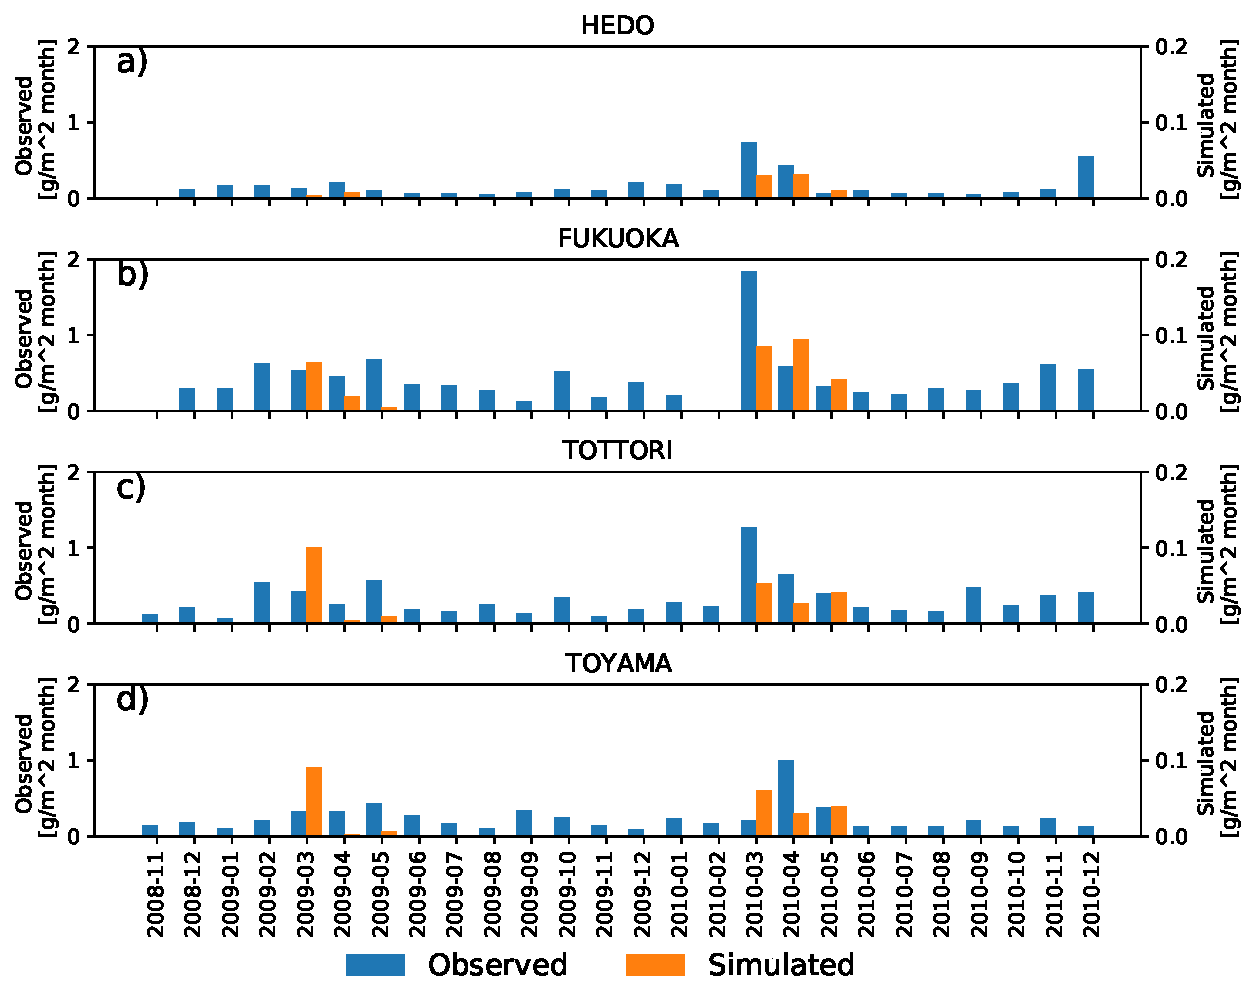
\includegraphics[width=\textwidth]{texfiles/figs/monthly_accumulated_dry_depostion_japan.pdf}
    \caption{Dry deposition of dust simulated at 4 locations by the coast of japan. The measurements of monthly deposition flux are described by \textcite{osada2014wet}}
    \label{fig:model_eval_dry_deposition}
\end{figure}

\begin{figure}[hptb]
    \centering
    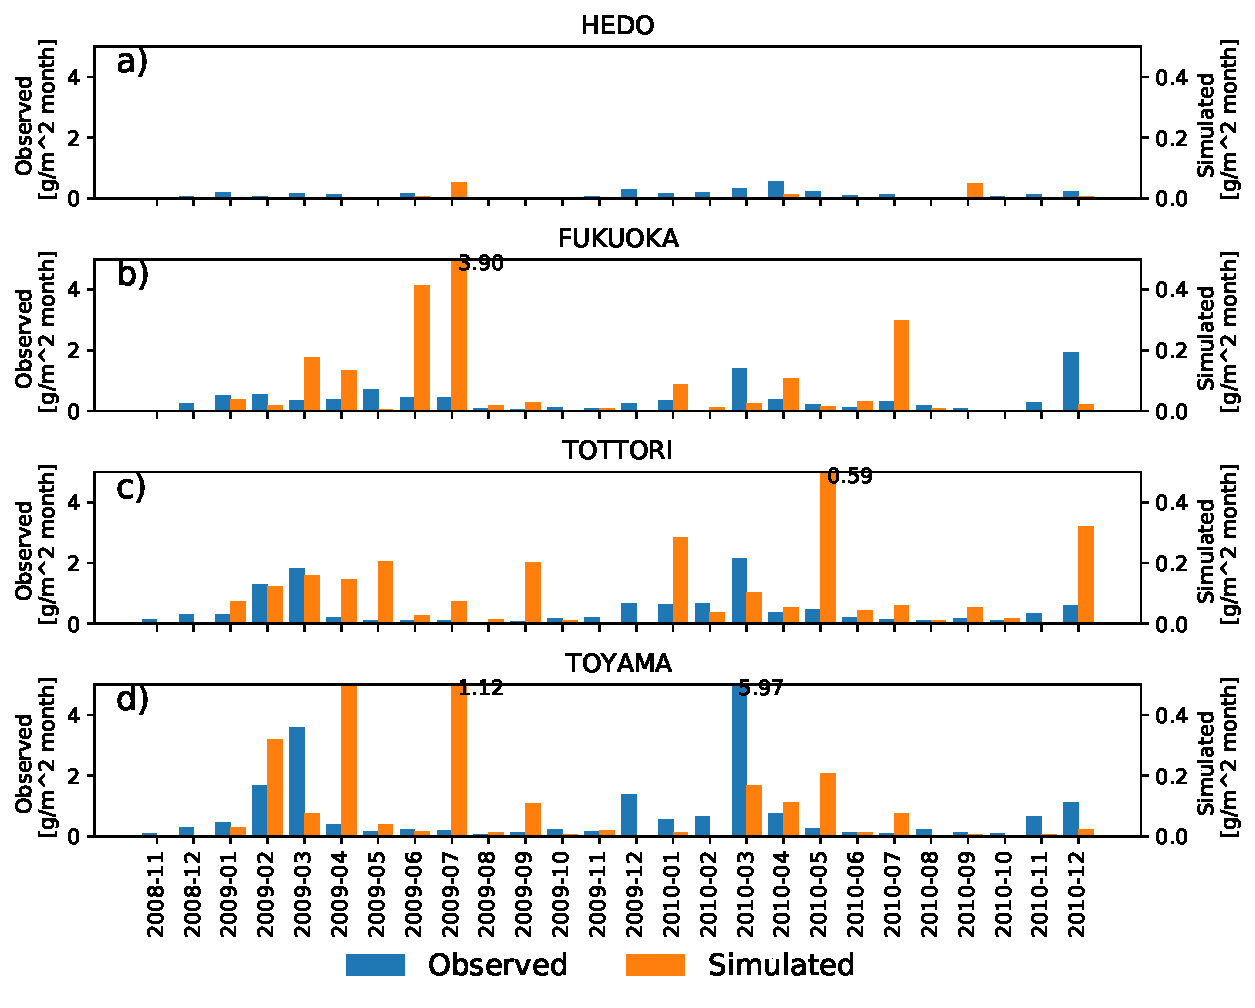
\includegraphics[width=\textwidth]{texfiles/figs/monthly_accumulated_wet_depostion_japan.pdf}
    \caption{Wet deposition of dust simulated at 4 locations of the coast of japan. The measurements of monthly deposition flux are described by \textcite{osada2014wet}}
    \label{fig:model_eval_wet_deposition}
\end{figure}

\section{Average dust emissions, transport and deposition}\label{sec:result_average}
To give some context to the investigation of the inter annual variation of dust emissions, transport and deposition in the \Cref{sec:inter_annual_results}. The average mode of dust emission, transport and deposition is examined first. 
\subsection{Dust emissions}
In the subsequent analysis the source regions are divided into five regions as shown in \Cref{fig:emission_map_flexdust}. The average spring time emission amount and percentage for the three source regions with the strongest emissions are shown \Cref{tab:emissions}. The estimated mean total spring emissions are 20.02 Mt/spring and are close to the estimates by \textcite{xuan2004identification} for PM30 of 27.6 Mt/year. 
\Cref{fig:emission_map_flexdust} shows the 20 year average of spring time dust emissions as simulated by FLEXDUST.
% The regions with the highest spring emission are identified as the arid regions north west of the \acrshort{clp},  (mean emissions of $6.12\si{Mt}/ \mathrm{spring}$), Taklamakan desert (mean emissions of $4.33\si{Mt} / \mathrm{spring}$) and Mongolia (mean emissions of $2.91\si{Mt} / \mathrm{spring}$). Additional minor dust sources include the Junggar Basin in the north west of China and the Qaidam Baisin close to the Tibetan plateau.  


\begin{table}[htpb]
\caption{The mean emissions per spring for the three largest source regions}
\centering
\begin{tabular}{@{}
>{\columncolor[HTML]{FFFFFF}}l 
>{\columncolor[HTML]{FFFFFF}}l 
>{\columncolor[HTML]{FFFFFF}}l @{}}
\toprule
 &  Emissions (Mt) &  Percentage (\%)\\ \midrule
Taklamakan & 4.330 & 21.6 \\
North west \acrshort{clp} &  6.117 & 30.5 \\
Mongolia &  2.913  & 14.4  \\
Remaining regions &  6.64 & 33.5 \\
Total &  20.02 & 100 \\ \bottomrule
\end{tabular}
\label{tab:emissions}
\end{table}


\begin{figure}[hptb]
    \centering
    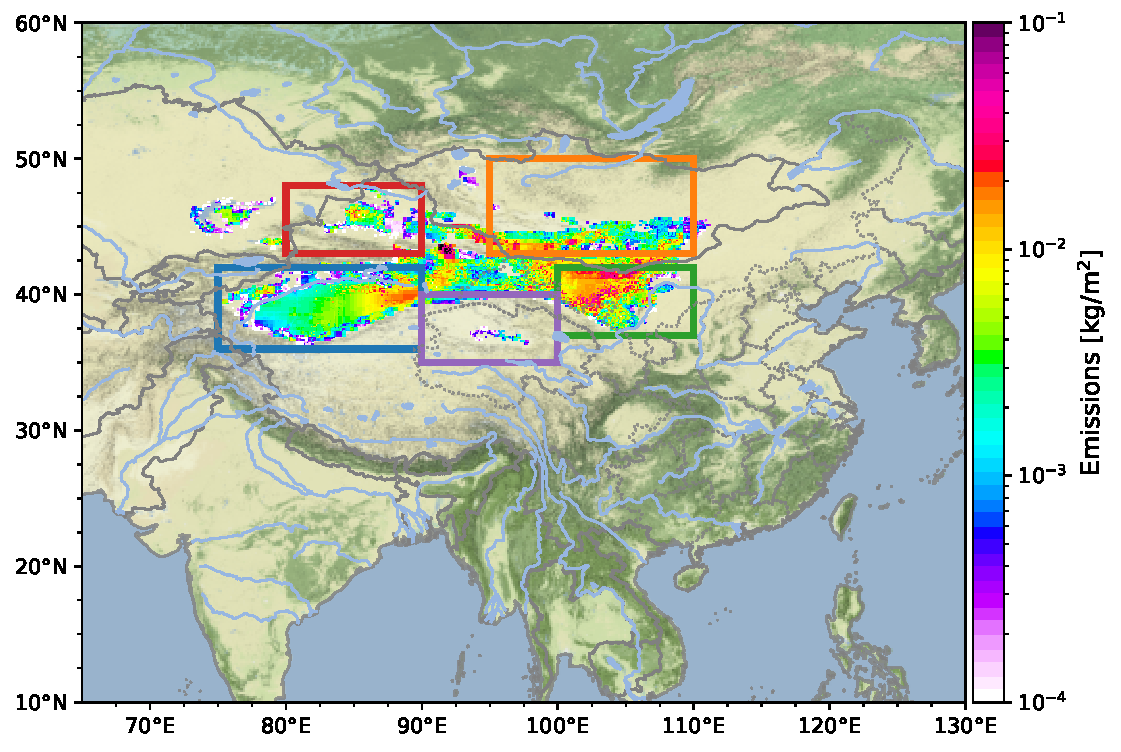
\includegraphics[width=\textwidth]{../figs/emission_map_1999_2019.pdf}
    \caption{Map of spring averaged dust emission flux simulated by FLEXDUST. The major source regions are indicated,  Junggar Basin \emph{(Red)},  Taklamakan (\emph{Blue}),  Qaidam Basin (\emph{Purple}), North west CLP (\emph{Green}),  Mongolia \emph{(Orange)}}
    \label{fig:emission_map_flexdust}
\end{figure}

\subsection{Dust Transport}
Mean dust loading transport trajectories for every location are shown in \Cref{fig:dust_loading_trajecs}. The average dust loading trajectories are calculated based on the centriod trajectory of each particle release and in the averaging procedure each centriod trajectory are given a weight based on their dust loading.  \Cref{fig:dust_loading_trajecs}a and b shows the averaged dry deposition dust loading trajectories for the fine clay and coarse silt particles respectively, with their accompanying vertical profiles shown in \Cref{fig:dust_loading_trajecs}c and d. Similarly wet deposition dust loading trajectories are shown in \Cref{fig:dust_loading_trajecs}e - h. The red points in \Cref{fig:dust_loading_trajecs} are spaced equally 12 hours apart and to indicate the velocity of dust transporting air masses. 
\begin{figure}[hptb]
    \centering
    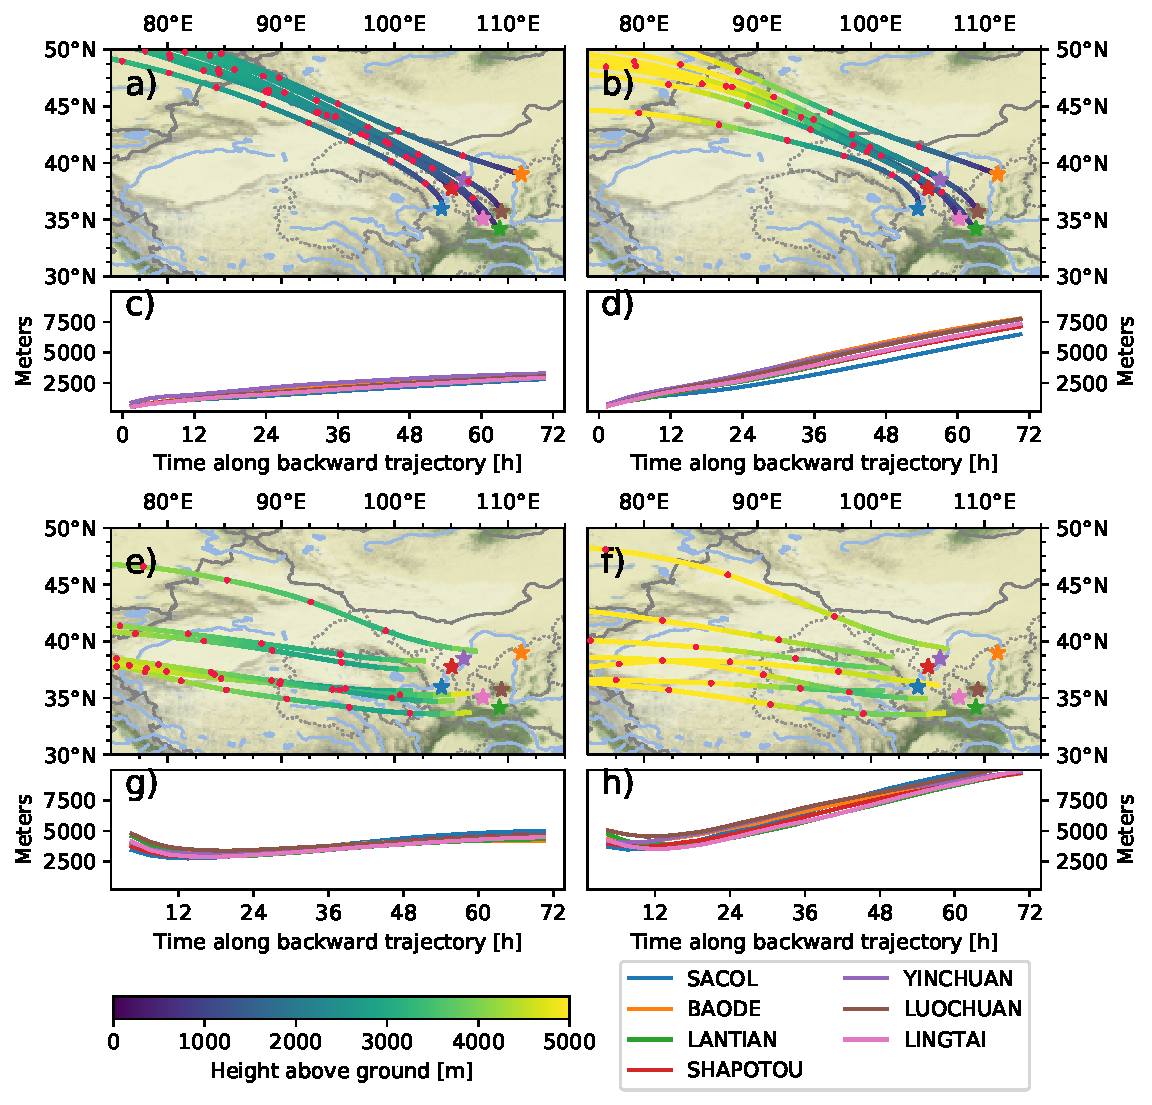
\includegraphics[width=\textwidth]{texfiles/figs/average_dust_transport_trajectories.pdf}
    \caption{Weighted average of centriod dust loading trajectories for all the receptor locations during springtime from 1999-2019. (a) and (b) is the dry deposition dust loading trajectories for "Fine clay" and "Coarse silt" respectively, (c) and (b) is their accompanying vertical path.  (e)-(f) as (a)-(b) just for wet deposition dust loading trajectories. The red points are spaced at 12 hours apart indicating the speed of the dust transporting airmasses }
    \label{fig:dust_loading_trajecs}
\end{figure}

Dry deposited dust of both particle size bins are primarily transported along a north easterly path. 
By comparison wet deposited dust are transported by air masses that originates from a more southerly direction. The coarse particles are on average transported by faster moving air masses compared to the fine dust particles as indicated by the distance between the red points.     

The vertical profile of the averaged trajectories shows that altitude of the dry deposited dust approximately decreases linearly with time. The height of the fine dust particles decreases more slowly with time compared to the coarser dust particles. This is suggest that for coarse dust to be transported from the remote source regions to the receptors would have to involve upper tropospheric transport. In contrast the fine dust particles are primarily transported through the lower troposphere regardless of the proximity of the source. This is also consistent with the coarse dust being transported more swiftly.  

The wet deposited dust as opposed to the dry deposited dust experience lifting starting approximately 12 hours before arriving at the receptor. Precipitation over the \acrshort{clp} during spring is usually caused by convection initiated by frontal activity. \Cref{fig:dust_loading_trajecs}g-h gives then an estimate of when when this frontal activity occurs and how long before being deposited at the receptor the dust needs to be entrained into the atmosphere.  
\subsection{Dust deposition}
\begin{figure}[htbp]
    \centering
    \includegraphics[width=\textwidth]{texfiles/figs/2micron_total_depositon_source_contribution.pdf}
    \caption{Yearly averaged spring source contribution "Fine Clay" dust size bin for the seven sites across the CLP (a-g). (h) shows the averaged spring deposition of each site for both wet- and dry deposition}
    \label{fig:source_contrib_2mmu}
\end{figure}

The advantage of using this approach for modelling dust deposition is that it makes it possible to directly quantify how much each source region is contributing to the deposition at the receptor.   
\Cref{fig:source_contrib_2mmu} and \Cref{fig:source_contrib_20mmu} shows the spring averaged source contribution for total deposition of the coarse and fine particles respectively. The main source contributing to the deposition from all the location is the proximal deserts north west of the \acrshort{clp}.  The western sites, Shapotou, Yinchuan, Sacol and Lingtai have a stronger contribution from Taklamakan compared to the eastern site. \Cref{fig:source_contrib_2mmu}h and \Cref{fig:source_contrib_20mmu}h shows that the primary mode of deposition for all the sites is wet deposition. The wet deposition is even more dominating for the coarse particles. This is consistent with the coarse particle requiring to be transported through the upper troposphere as shown by the average dust loading trajectories considering that it is more likely that dust particles at higher altitudes will be subjected to cloud scavenging.     
 \begin{figure}[htbp]
    \centering
    \includegraphics[width=\textwidth]{texfiles/figs/20micron_total_depositon_source_contribution.pdf}
    \caption{Yearly averaged March-May source contribution "Coarse Silt" size bin for the seven sites across the CLP (a-g). Panel h) shows the averaged spring deposition of each site for both wet- and dry deposition}
    \label{fig:source_contrib_20mmu}
\end{figure}

\section{Inter-annual variations in emission, transport and deposition}\label{sec:inter_annual_results}

\subsection{Inter-annual variation in emissions}
The time series of spring time emissions for the 3 major source regions are shown in \Cref{fig:emission_timeseries}. Over this 20 year period there is no overall trend in the spring time emissions from the East Asian sources. The three years with the strongest overall dust emissions are identified as 2001, 2010 and 2018. For 2001 and 2010 the North west CLP regions stands for the largest increase in emissions, whereas for 2018 Taklamakan and the smaller source regions are mostly responsible for the increased emission. Years with strong emissions from the North west CLP and generally coincide with enhanced emissions from Mongolia but not always with enhanced emissions from Taklamakan, e.g. 2013.   

\begin{figure}[htbp]
    \centering
    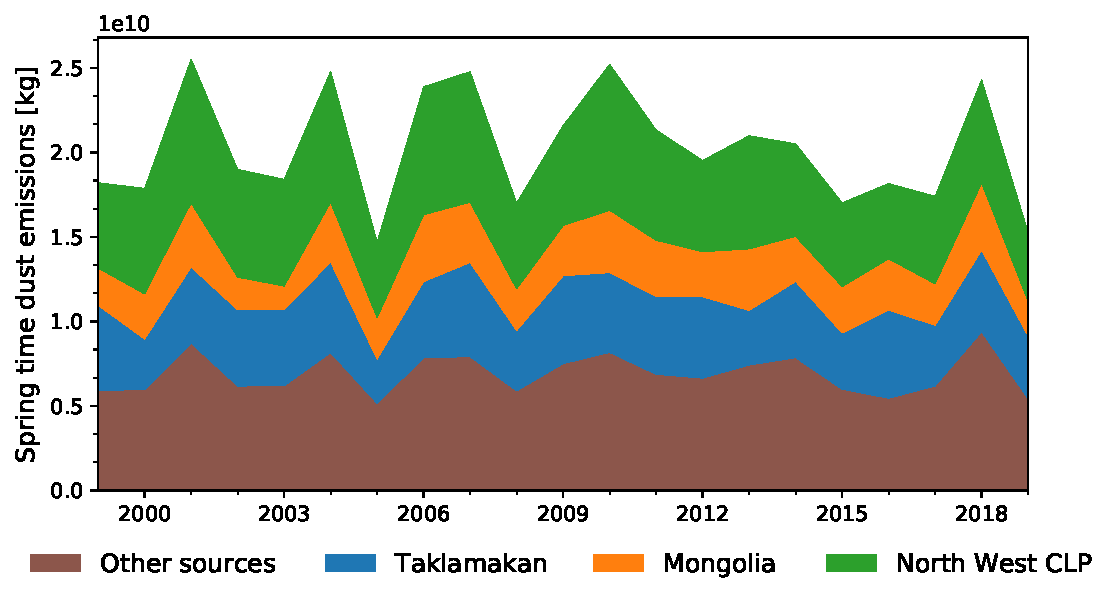
\includegraphics[width=\textwidth]{../figs/Emission_timeseries.pdf}
    \caption{Time series of total spring time dust emissions from 1999-2019. The total emission is partitioned into the contribution from the Taklamakan (Blue), North West CLP (Green) and Mongolia (Orange) }
    \label{fig:emission_timeseries}
\end{figure}

\acrfull{eof} analysis based on yearly de-trended spring emissions was done to identify the interannual variations in the spatiotemporal characteristics of spring dust emissions from East Asian deserts. The significance of each EOF was evaluated based on the rule of thumb outlined by \textcite{north1982sampling}. Stating that if the neighbouring eigenvalue lay within the typically error of the respective eigenvalue $\lambda$, the two EOFs might be mixed in their signal and hence not representing true patterns. Following this rule, \Cref{fig:eof_test} shows that the first and second \acrshort{eof} meets this criterion.  

\begin{figure}[htbp]
    \centering
    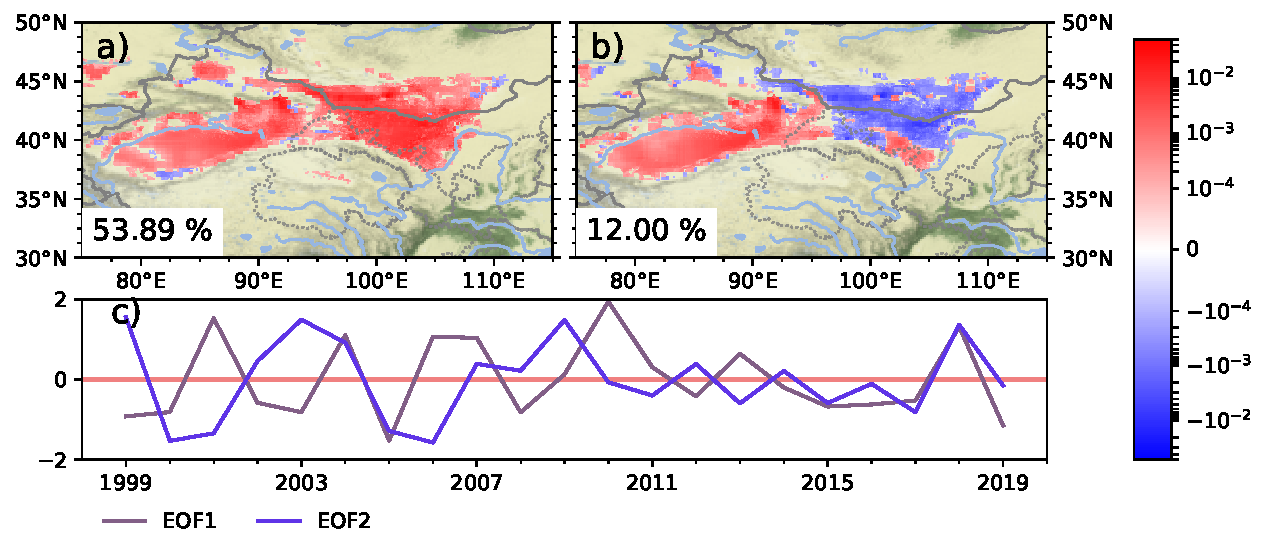
\includegraphics[width=\textwidth]{texfiles/figs/Emissions_EOF.pdf}
    \caption{The spatial pattern of the leading EOF (a) and second EOF (b). (c) the time series of the normalized principal component of the first (purple) and second (blue) EOFs.}
    \label{fig:emissions_eof}
\end{figure}
\Cref{fig:emissions_eof}a and b shows the spatial pattern of EOF1 and EOF2. EOF1 and EOF2 account for 54 \% and 12 \% of the total variance in annual spring time emissions. The leading EOF represent increased emissions across all the source regions and as expected the years with a large positive principal component (PC) correspond to to strong emissions years (\Cref{fig:emissions_eof}c). Interestingly the second EOF shows a dipole pattern between emissions in Mongolia and Taklamakan. The signal of the second EOF is also visible from the time series where the positive EOF2 years correspond to a disproportional increase in emissions from Taklamakan compared to emissions from Mongolia and vice versa.       

Composite analysis of the preceding winter circulation for strong positive minus strong negative EOF years was done in order to examine what kind of atmospheric circulation that is responsible for the spatial patterns identified by the \acrshort{eof} analysis. In positive EOF1 years the composite anomalies indicate a negative \acrshort{ao} mode, with positive \acrshort{mslp} anomalies over the arctic region. The composite anomalies for the second EOF show a weakened Aleutian low and Siberian high suggesting weak \acrshort{eawm} circulation. In other words the EOF analysis suggest increased emissions from Taklamakan during weak \acrshort{eawm} years.     
\begin{figure}[htpb]
    \centering
    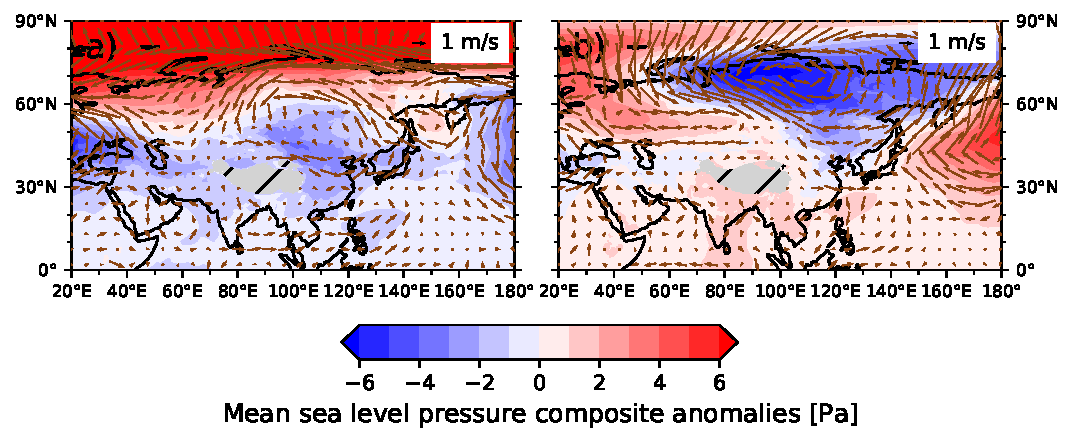
\includegraphics[width=\textwidth]{texfiles/figs/EOF_emissions_composite.pdf}
    \caption{DJF composite anomalies of MSLP and 850hPa winds the strong positive minus strong negative  EOF1 (a) and EOF2 (b) years}
    \label{fig:eof_composite_DJF}
\end{figure}
The MAM composite (\Cref{fig:eof_composite_MAM}b) shows how the circulation anomalies evolve into spring. In spring composite the circulation seems to have transitioned to more negative AO mode like circulation pattern with negative MSLP anomalies over the arctic region. Moreover there is now a weak negative pressure anomalies over Taklamakan producing enhanced winds intruding into the basin. The north easterly flow has also weakened, which could explain the reduction in emissions from the Mongolian region. 
\begin{figure}[htpb]
    \centering
    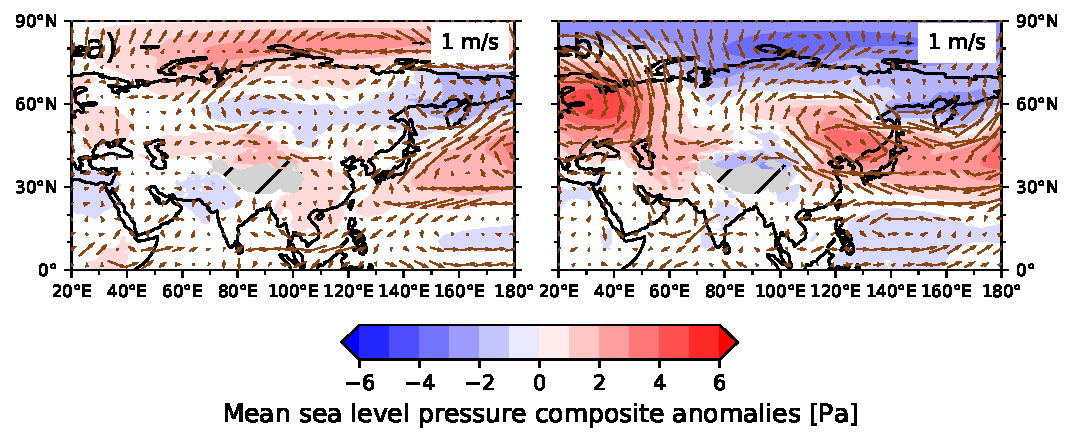
\includegraphics[width=\textwidth]{texfiles/figs/EOF_emissions_composite_MAM.pdf}
    \caption{\acrshort{mam} composite anomalies of MSLP and 850hPa winds the strong positive minus strong negative  EOF1 (a) and EOF2 (b) years}
    \label{fig:eof_composite_MAM}
\end{figure}

\subsection{Inter-annual variation in dust transport}
\begin{figure}[htbp]
    \centering
    \includegraphics[width=\textwidth]{texfiles/figs/2_micron_drydep_weak_strong_trajecs .pdf}
    \caption{The weighted average of dry deposited fine clay dust loading trajectories for strong and weak deposition years for every location. The standard deviation of the trajectories during the weak deposition and strong deposition years are represented by the blue and red shading respectively.  (h) show the difference in height of the dust transporting air masses during strong and weak deposition years. }
    \label{fig:strong_weak_drydepo_year_2mmu_trajecs}
\end{figure}

Examining the differences in transport between strong and weak deposition years helps to understand what kind of transport that is responsible for the increase \acrshort{mar} over the \acrshort{clp}. The differences in transport between the weak and strong deposition years for the all the receptor locations were examined by taking weighted mean of the centriod trajectories during weak and strong wet and dry deposition years for both the fine and coarse particle size bins. 
\Cref{fig:strong_weak_drydepo_year_2mmu_trajecs} and \Cref{fig:strong_weak_drydepo_year_20mmu_trajecs} shows the dry deposition dust loading trajectories for the fine and coarse particle size bin respectively. 
The standard deviation during strong years and weak years are shaded red and blue respectively and the purple region is where the two overlap. During the strong deposition years the spread is generally narrower and condensed in a north easterly direction.  In addition the dust transporting airmasses are moving more swiftly compared to the weak deposition years. 
The dust transport is generally happening at higher altitudes during the strong deposition years. The exception being transport of fine dust to Shapotau and Sacol, which are located in close proximity to the sources regions. This suggest that dry deposition of fine dust at these location might be most favourable during moderate dust events.


\begin{figure}[htbp]
    \centering
    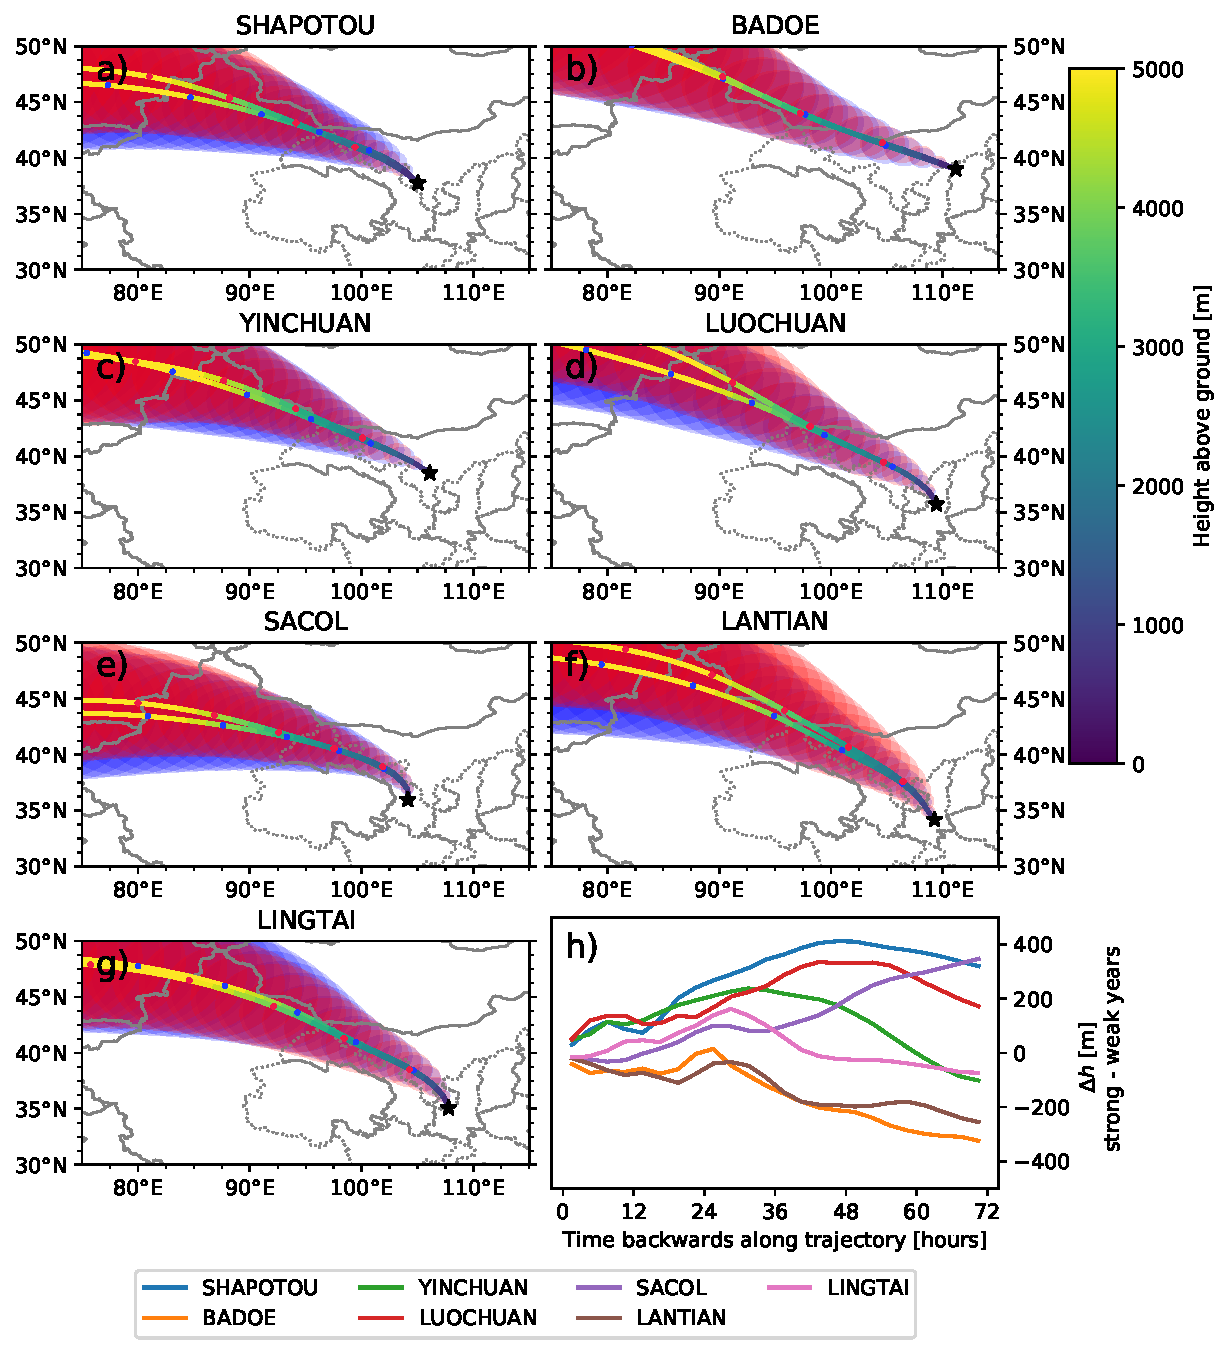
\includegraphics[width=\textwidth]{texfiles/figs/20_micron_drydep_weak_strong_trajecs.pdf}
    \caption{The weighted average of dry deposited coarse silt dust loading trajectories for strong and weak deposition years for every location. The standard deviation of the trajectories during the weak deposition and strong deposition years are represented by the blue and red shading respectively.  (h) show the difference in height of the dust transporting air masses during strong and weak deposition years. }
    \label{fig:strong_weak_drydepo_year_20mmu_trajecs}
\end{figure}

Due to the prerequisites needed for wet deposition to occur is a more random process and not strongly influenced by changes in the mean winds, the interpretation of the difference in wet deposition path are more difficult to interpret. 
\begin{figure}[htbp]
    \centering
    \includegraphics[width=\textwidth]{texfiles/figs/2_micron_wetdep_weak_strong_trajecs.pdf}
    \caption{The weighted average of wet deposited fine clay dust loading trajectories for strong and weak deposition years for every location. The standard deviation of the trajectories during the weak deposition and strong deposition years are represented by the blue and red shading respectively.  (h) show the difference in height of the dust transporting air masses during strong and weak deposition years. }
    \label{fig:strong_weak_wetdepo_year_2mmu_trajecs}
\end{figure}

\begin{figure}[htbp]
    \centering
    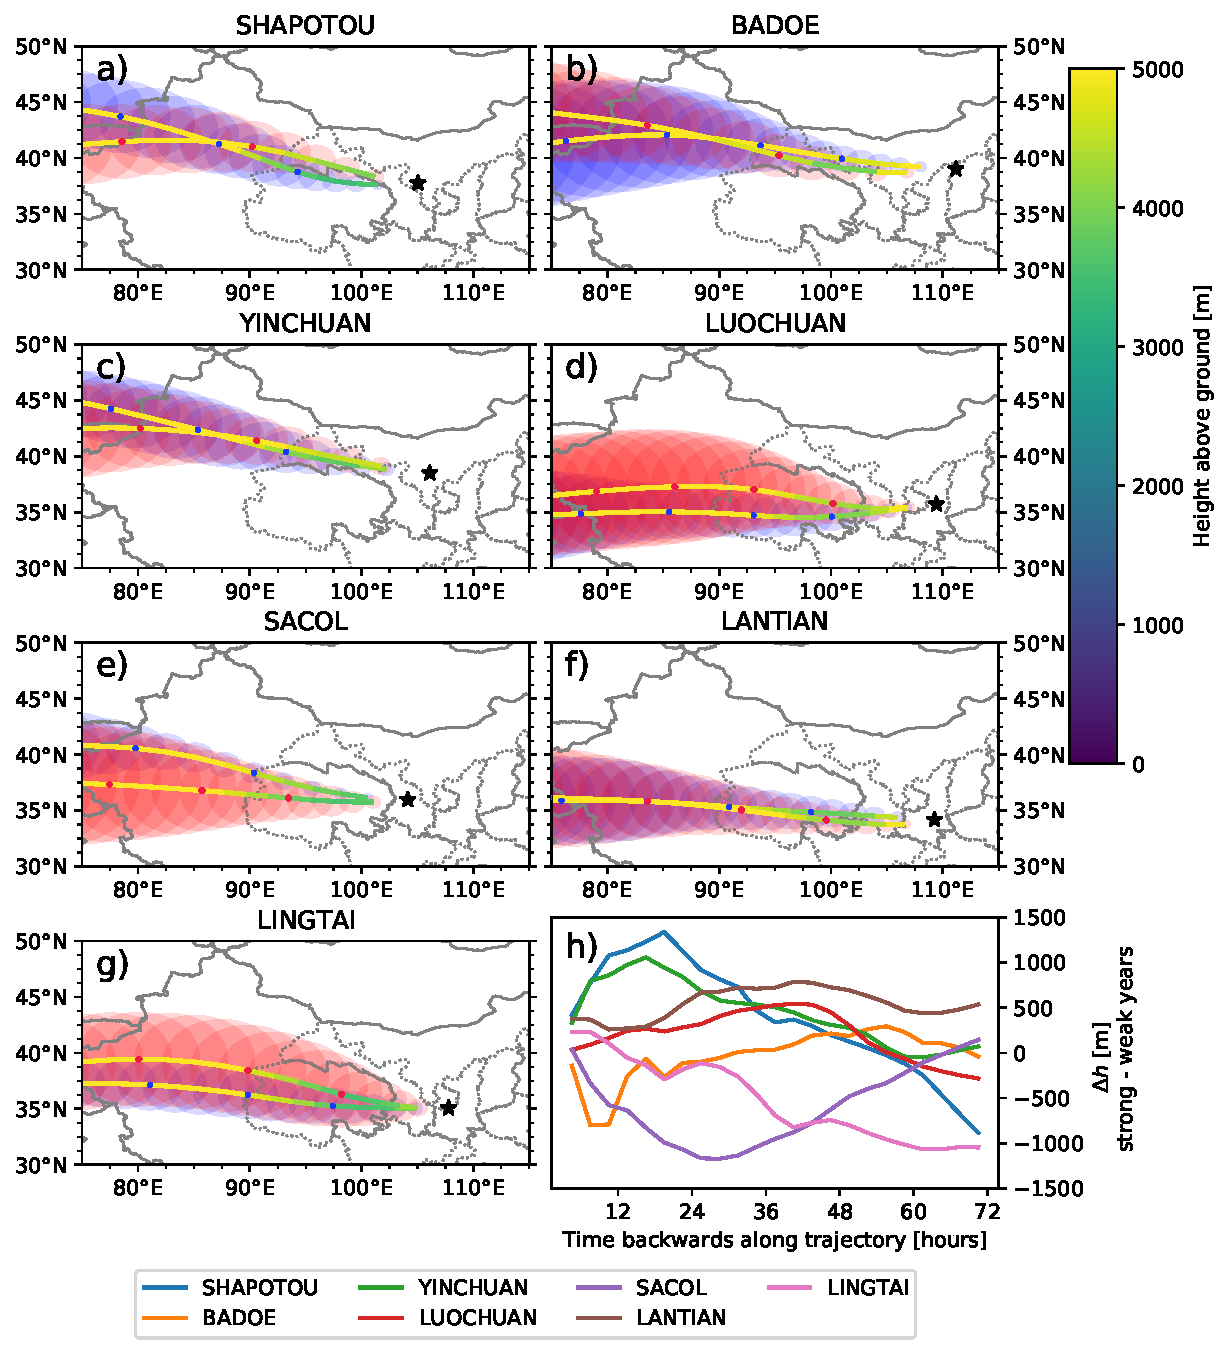
\includegraphics[width=\textwidth]{texfiles/figs/20_micron_wetdep_weak_strong_trajecs.pdf}
    \caption{The weighted average of wet deposited coarse silt dust loading trajectories for strong and weak deposition years for every location. The standard deviation of the trajectories during the weak deposition and strong deposition years are represented by the blue and red shading respectively.  (h) show the difference in height of the dust transporting air masses during strong and weak deposition years. }
    \label{fig:strong_weak_wetdepo_year_20mmu_trajecs}
\end{figure}

\subsection{Inter annual variation in source contribution}
\begin{figure}[hptb]
    \centering
    \includegraphics[width=\textwidth]{texfiles/figs/composite_source_contrib_2micron_tot_dep.pdf}
    \caption{Normalised source contribution composite anomalies of "fine clay" particle size bin for all locations, strong - weak deposition years.}
    \label{fig:source_contrib2mmu_anomalies}
\end{figure}
From the mineralogy of the loess deposits it is possible to differentiate the provenance of deposited dust in periods of high and weak \acrshort{mar}. Conversely the similar question can be examined with FLEXPART by comparing the source contribution during weak and strong deposition years.  
\Cref{fig:source_contrib2mmu_anomalies} shows the normalised source contribution for the "fine clay" particle size bin. The model result suggests that strong deposition years have more concentrated source contribution. The exception is Sacol (\Cref{fig:source_contrib2mmu_anomalies}e) which during strong deposition years has increased contribution from the entire region north west of the \acrshort{clp}. The more concentrated source contribution during strong deposition years suggest that the strong deposition years are set apart from the weak deposition years by having a large contribution from single strong dust event. By comparison the weak deposition years the source regions are more randomly distributed. \Cref{fig:source_contrib20mmu_anomalies} is as the previous figure just for the "coarse silt" particle size bin and tells much of the same message. However Lantian which has reduced  deposition from Taklamakan during strong deposition years for the fine particle size bin show increased contribution from Taklamakan during strong deposition years.      
\begin{figure}[hptb]
    \centering
    \includegraphics[width=\textwidth]{texfiles/figs/composite_source_contrib_20micron_tot_dep.pdf}
    \caption{Normalised source contribution composite anomalies of "coarse silt" particle size bin for all locations, strong - weak deposition years.}
    \label{fig:source_contrib20mmu_anomalies}
\end{figure}

\subsection{Inter annual correlations among deposition at each site and local and large-scale climate indices}
To analyse the effect of regional and large scale circulation circulation changes on the strength of the deposition over the \acrshort{clp}. Correlation analysis between deposition at each site and several indices of representing the \acrshort{eawm} strength as well as the \acrshort{ao}. The circulation indices are derived from seasonal averaged ERA5 reanalysis. The full analysis is shown in \Cref{fig:correlations} where the significant values are displayed. The winter \acrshort{ao} and \acrshort{nao} show the strongest correlation with dust deposition of all the indices considered in this analysis. Contradictory to previous research there is only a very weak correlation between the \acrshort{eawm} and deposition. 

\begin{figure}[htpb]
    \centering
    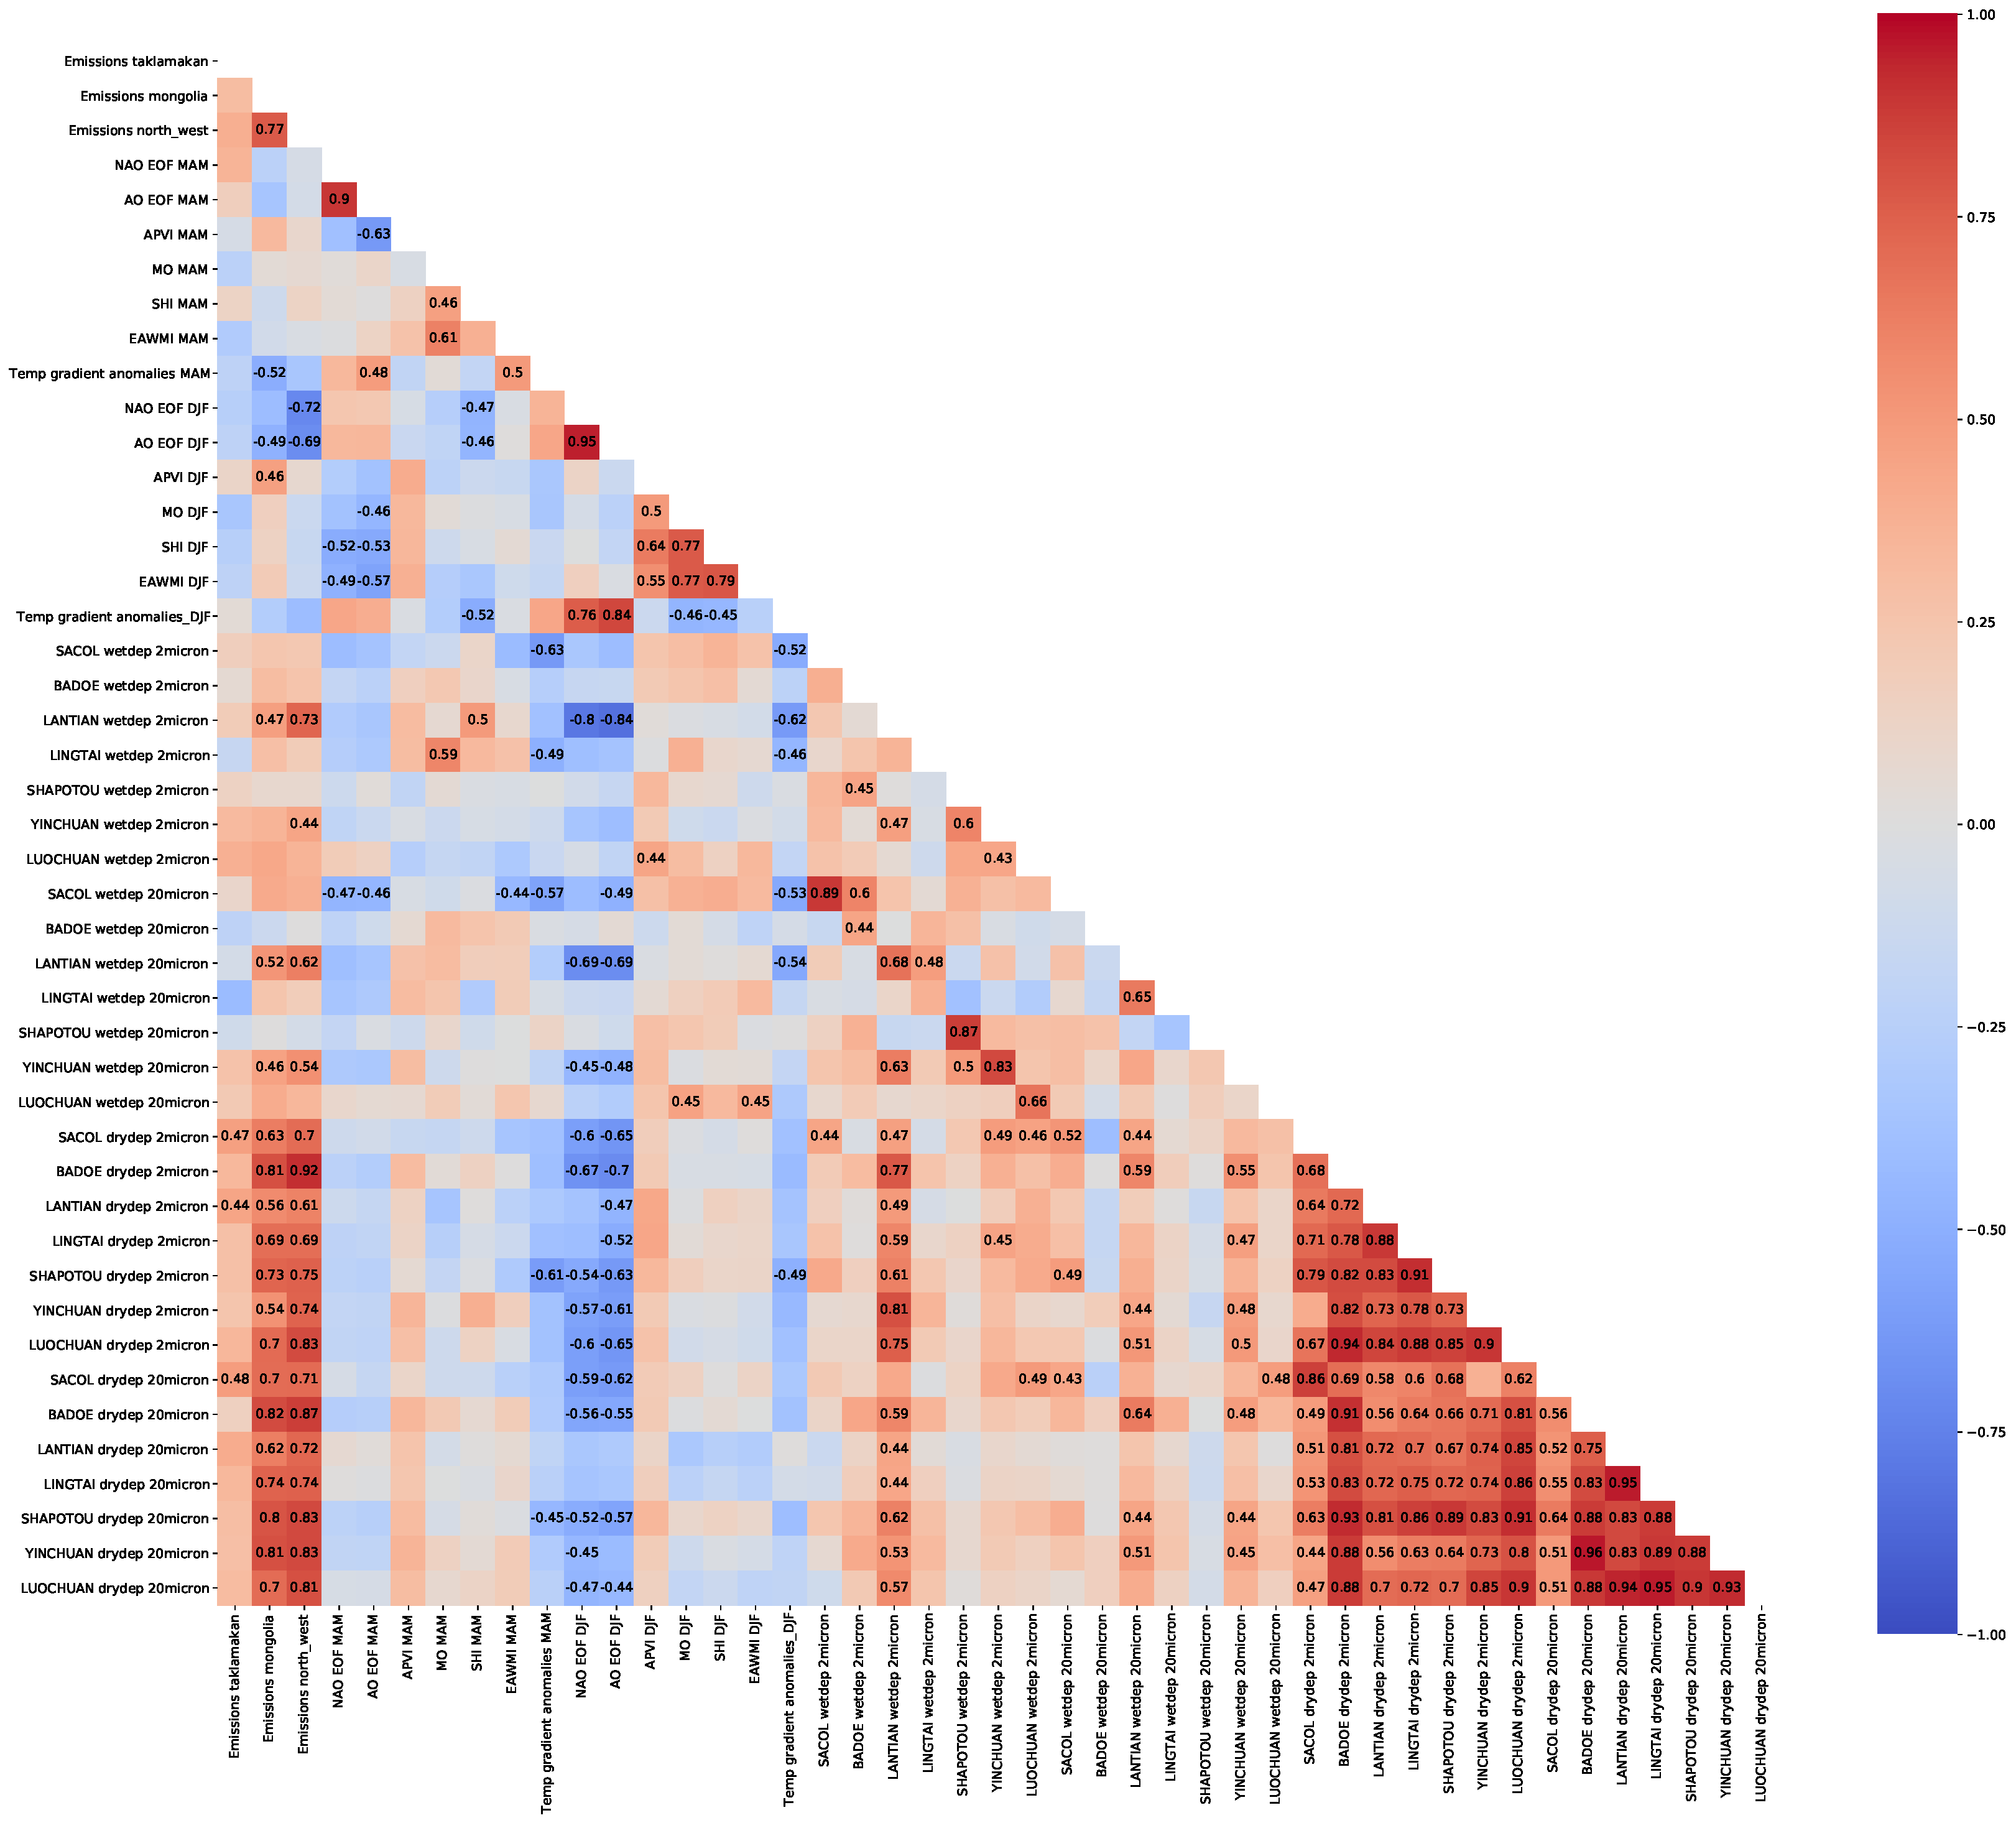
\includegraphics[width=\textwidth]{texfiles/figs/correlations.pdf}
    \caption{Inter annual correlations between deposition and each site and local and large-scale climate indices. The significant correlations are indicated}
    \label{fig:correlations}
\end{figure}

To examine how variations in the emission strength at the different source regions are reflected in the deposition at the receptor locations correlation analysis between deposition and emissions were also conducted. The correlation analysis (\Cref{fig:correlations}) show that dry deposition at almost all of the sites is strongly correlated with emissions in Mongolia and the north west \acrshort{clp}. However only Lantian and SACOL show a significant correlation between emissions from Taklamakan and dry deposition. Moreover wet deposition generally show a strong correlation between depostion and emissions for all of the sites. This exemplifies the randomness of the occurrence of wet deposition events. 

The correlations between deposition among the sites, show that wet deposition at Lantian correlates well with dry deposition at almost all the other sites. 

\subsection{Circulation composites}

To better understand the circulation differences between strong and weak deposition years composite differences anomalies were calculated by subtracting the circulation during strong minus weak deposition years. The circulation anomalies of \acrshort{djf} 850hPa winds and \acrshort{mslp} are shown in \Cref{fig:DJF_850_fine_composite} and \Cref{fig:DJF_850_coarse_composite} for the fine and coarse particles respectively. Comparing the composite anomalies to the composite anomalies of strong \acrshort{ao} (\Cref{fig:mo_ao_composite}a) and \acrshort{eawm} (\Cref{fig:mo_ao_composite}b) the deposition composites are generally consistent with negative ao circulation anomalies. The exception being Badoe which seems be strongly influencde by the ocean. 


\begin{figure}[hp]
    \centering
    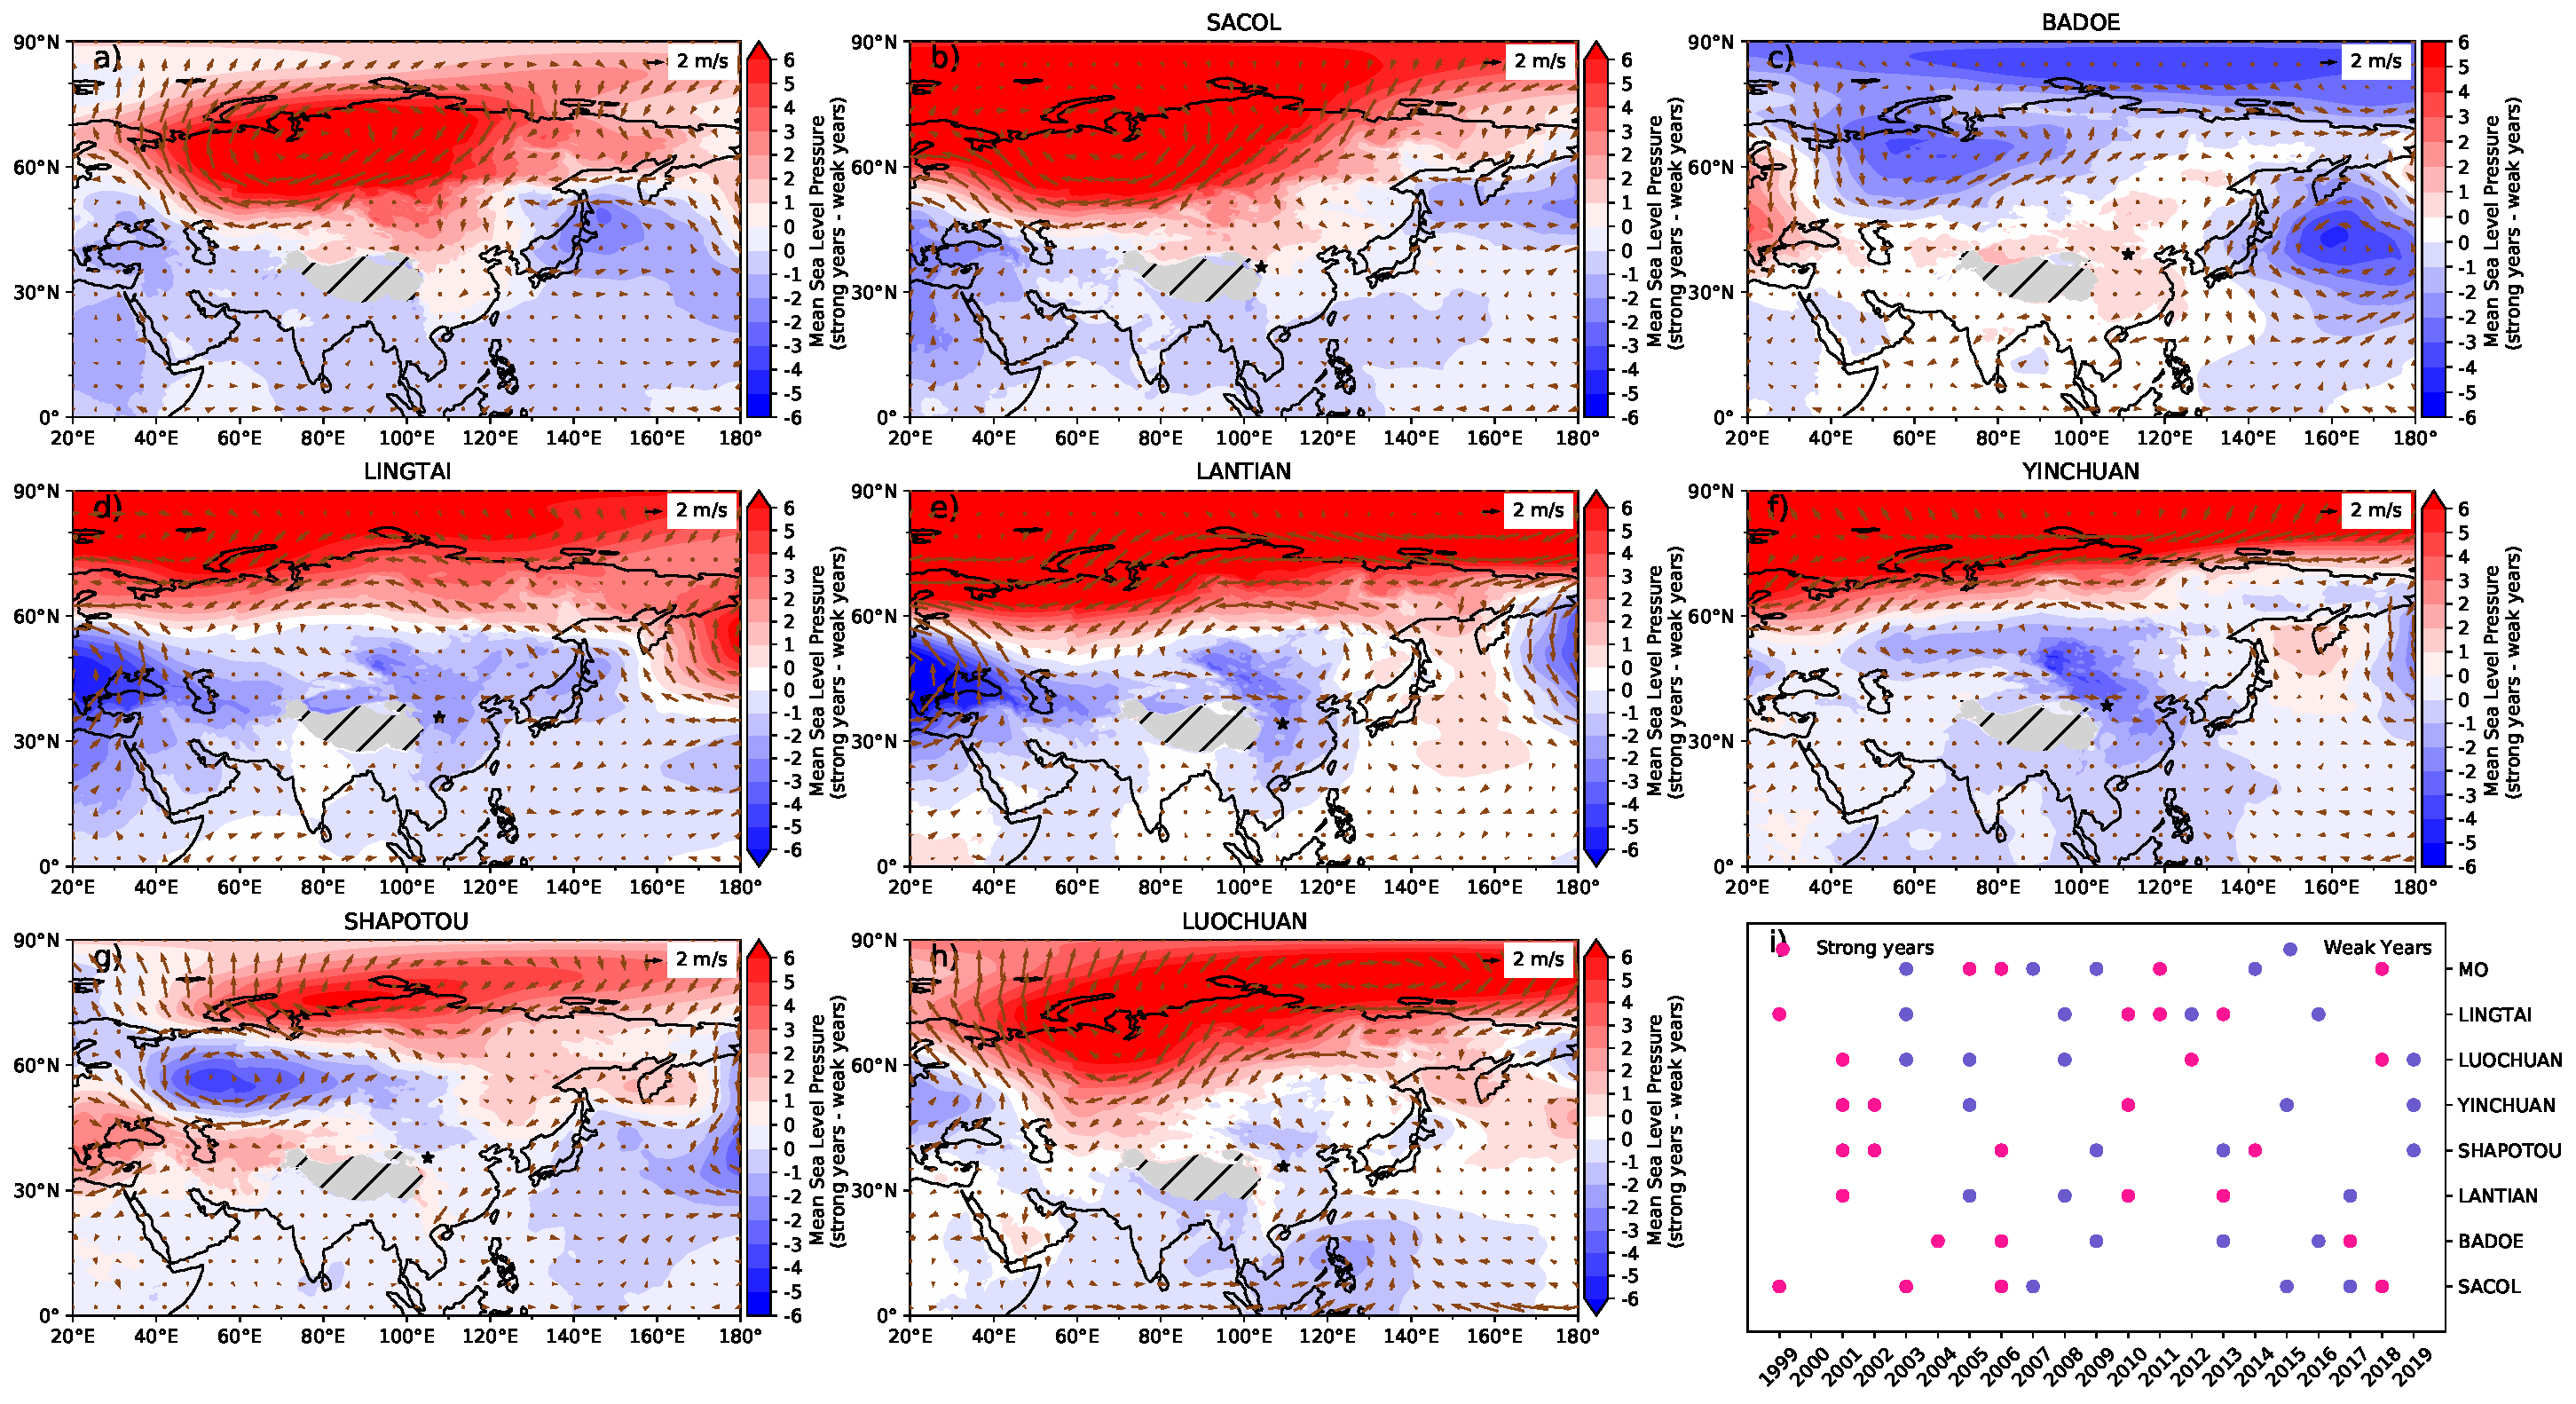
\includegraphics[width=\columnwidth]{texfiles/figs/mslp_850hPa_2micron_DJF.pdf}
    \caption{Composite difference anomalies of mean sea level pressure and 850hPa strong minus weak deposition years of the "fine clay" size bin in winter (DJF) for all the locations (a-g). (h) indicates which years are strong years and which years are weak.}
    \label{fig:DJF_850_fine_composite}
\end{figure}

\begin{figure}[hp]
    \centering
    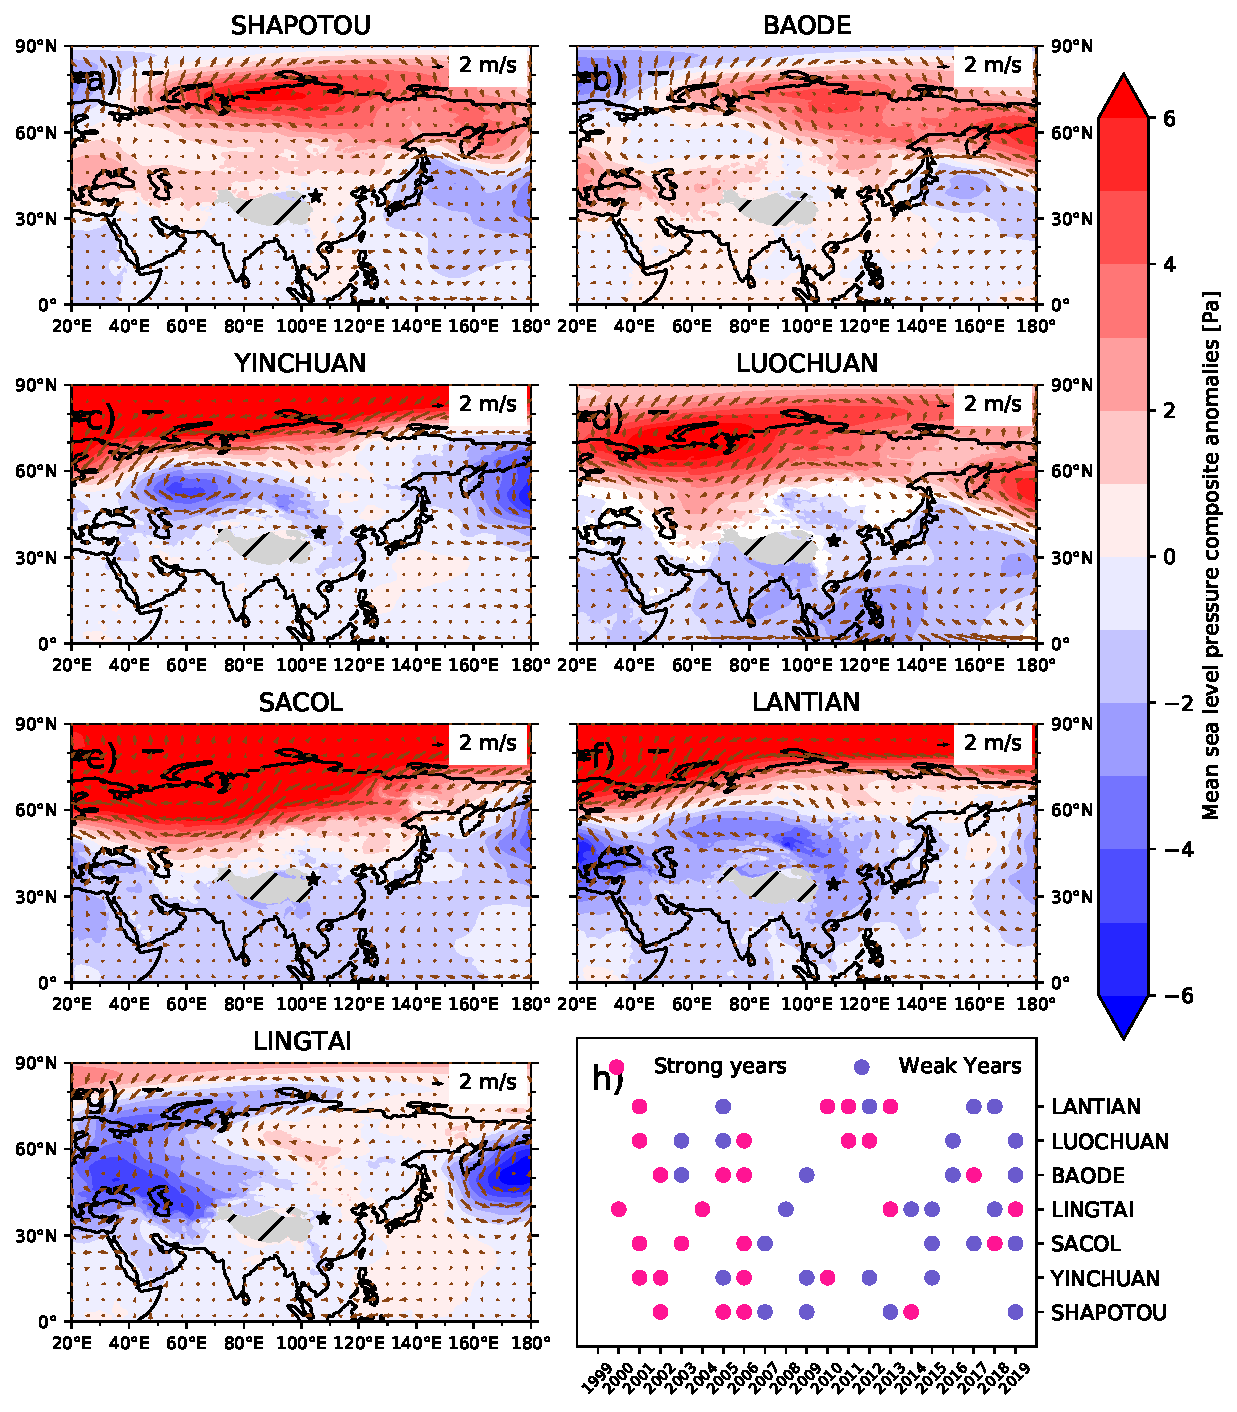
\includegraphics[width=\textwidth]{texfiles/figs/mslp_850hPa_20micron_DJF.pdf}
    \caption{Composite difference anomalies of mean sea level pressure and 850hPa strong minus weak deposition years of the "coarse silt" size bin in winter (DJF) for all the locations (a-g).  (h) indicates which years are strong years and which years are weak.}
    \label{fig:DJF_850_coarse_composite}
\end{figure}

\begin{figure}[htbp]
    \centering
    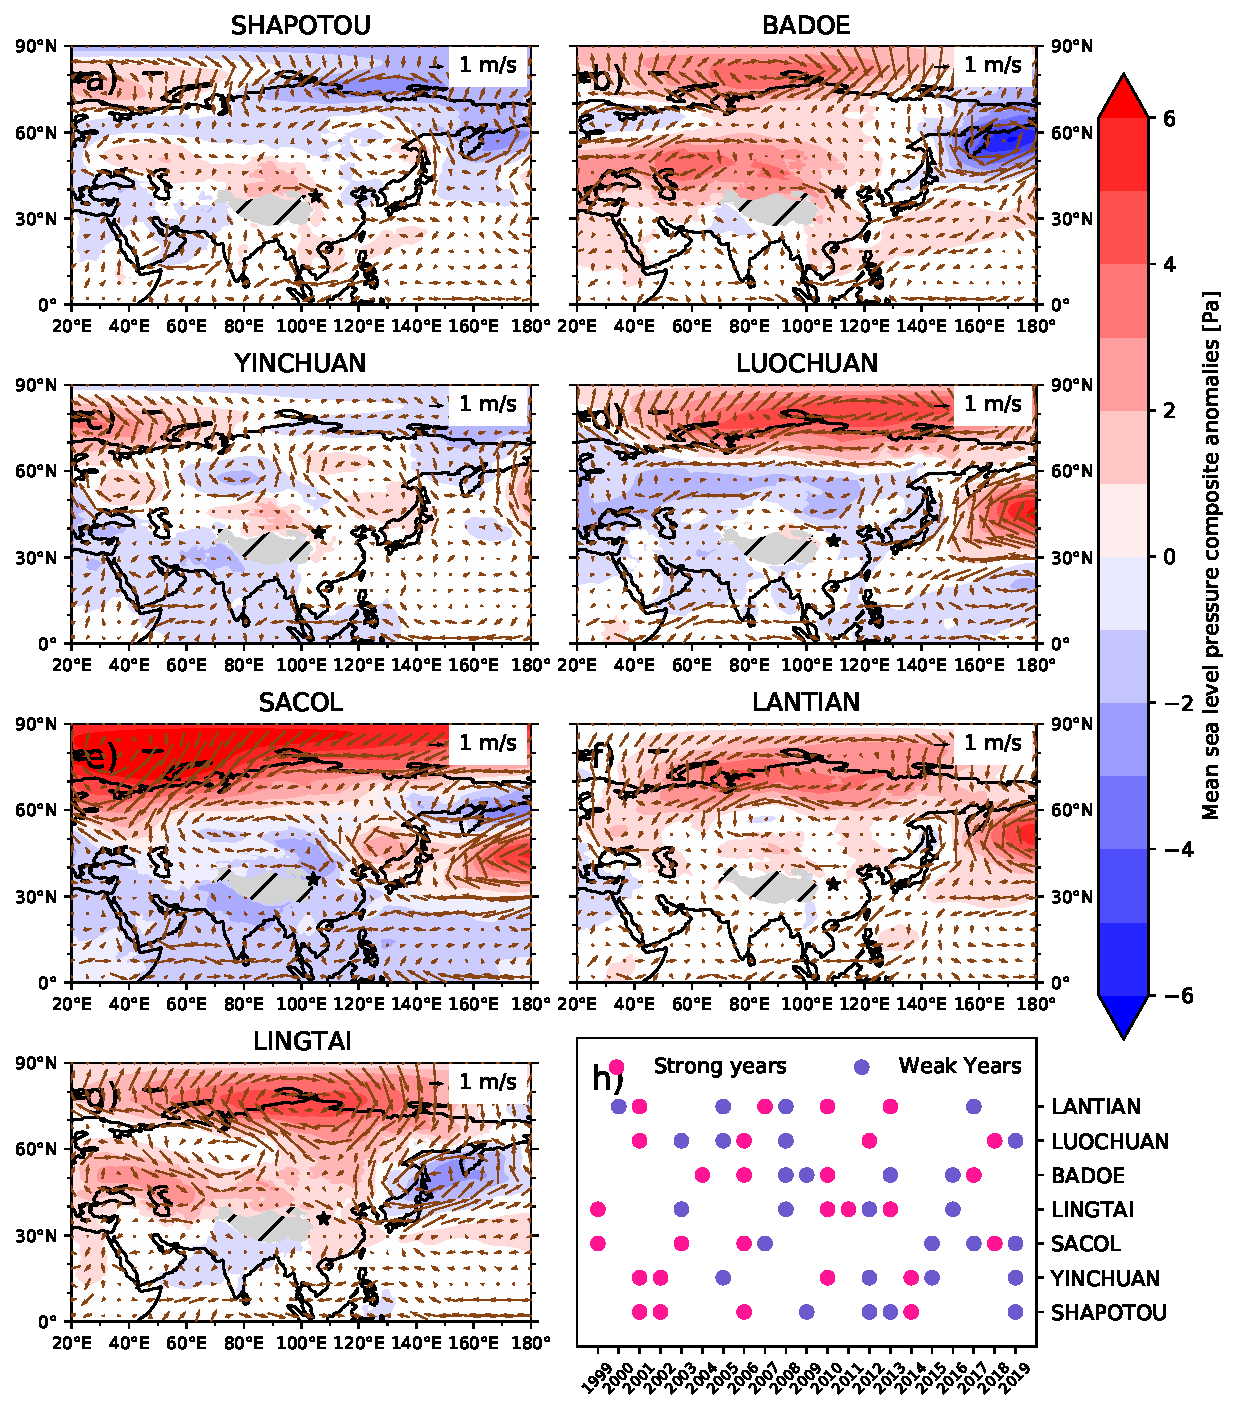
\includegraphics[width=\textwidth]{texfiles/figs/mslp_850hPa_2micron_MAM.pdf}
    \caption{Composite difference anomalies of mean sea level pressure and 850hPa strong minus weak deposition years of the "fine clay" size bin in spring (MAM) for all the locations (a-g).  (h) indicates which years are strong years and which years are weak.}
    \label{fig:MAM_850_fine_composite}
\end{figure}

\begin{figure}[htbp]
    \centering
    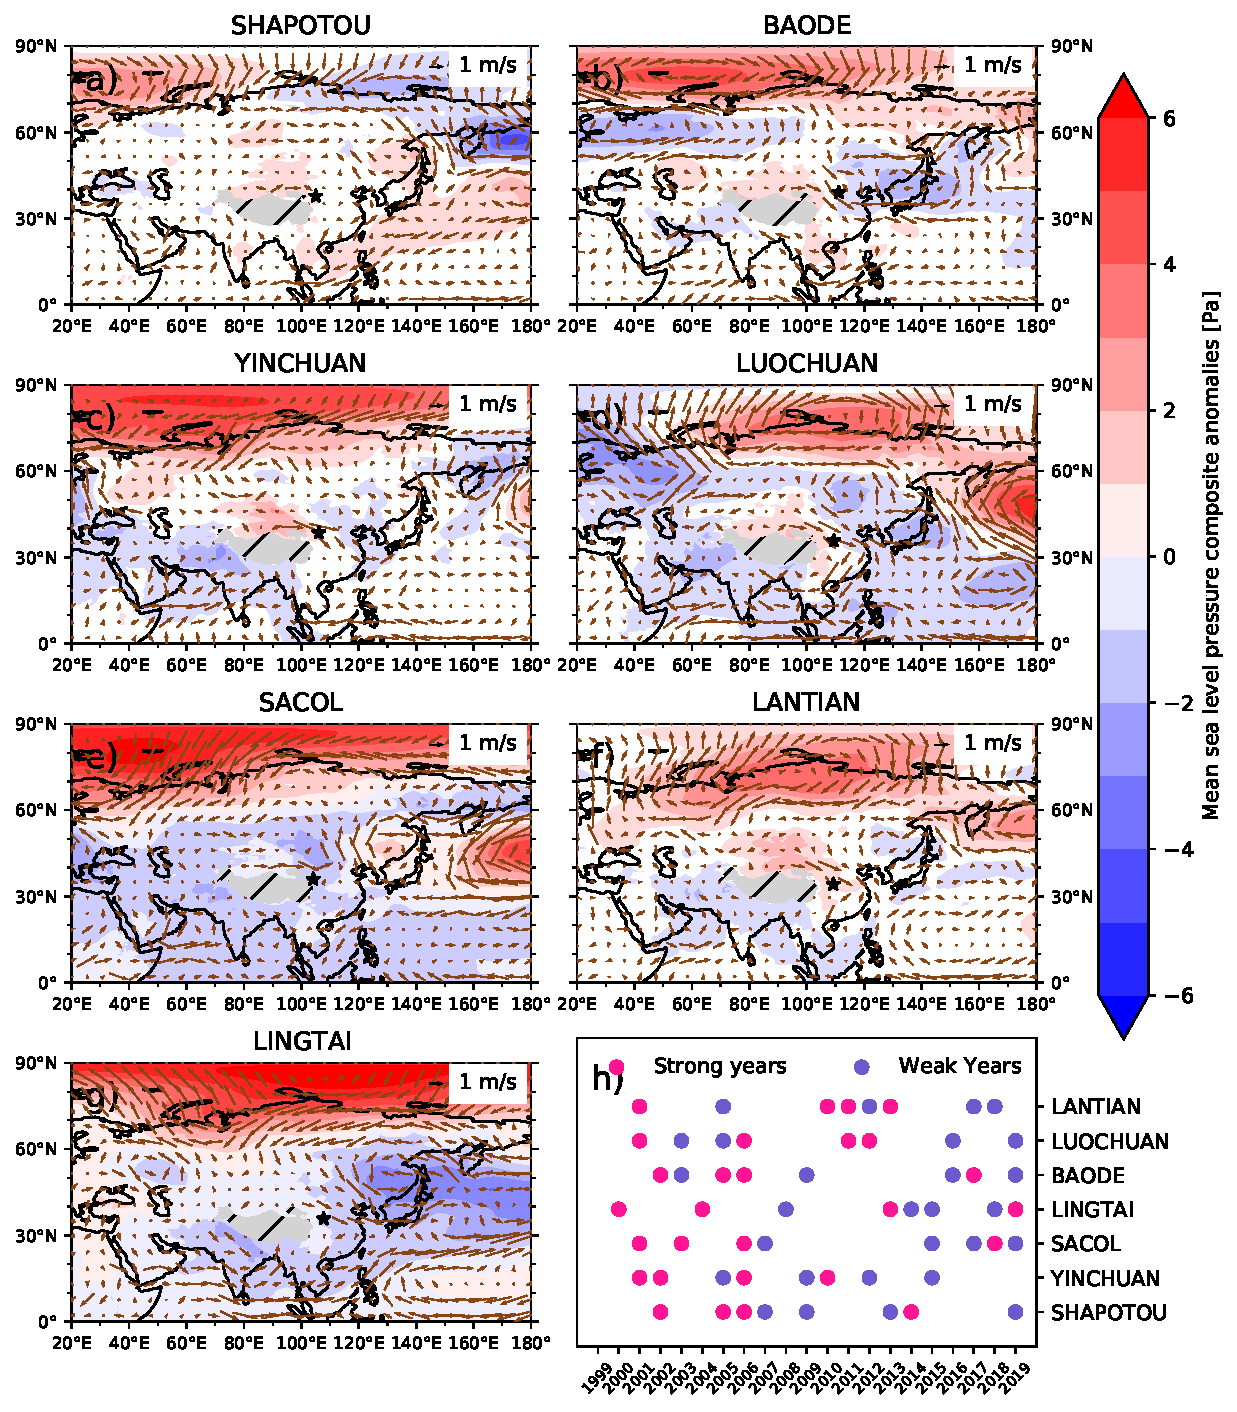
\includegraphics[width=\textwidth]{texfiles/figs/mslp_850hPa_20micron_MAM.pdf}
    \caption{Composite difference anomalies of mean sea level pressure and 850hPa strong minus weak deposition years of the "coarse silt" size bin in spring (MAM) for all the locations (a-g).  (h) indicates which years are strong years and which years are weak.}
    \label{fig:MAM_850_coarse_composite}
\end{figure}


\begin{figure}[hptb]
    \centering
    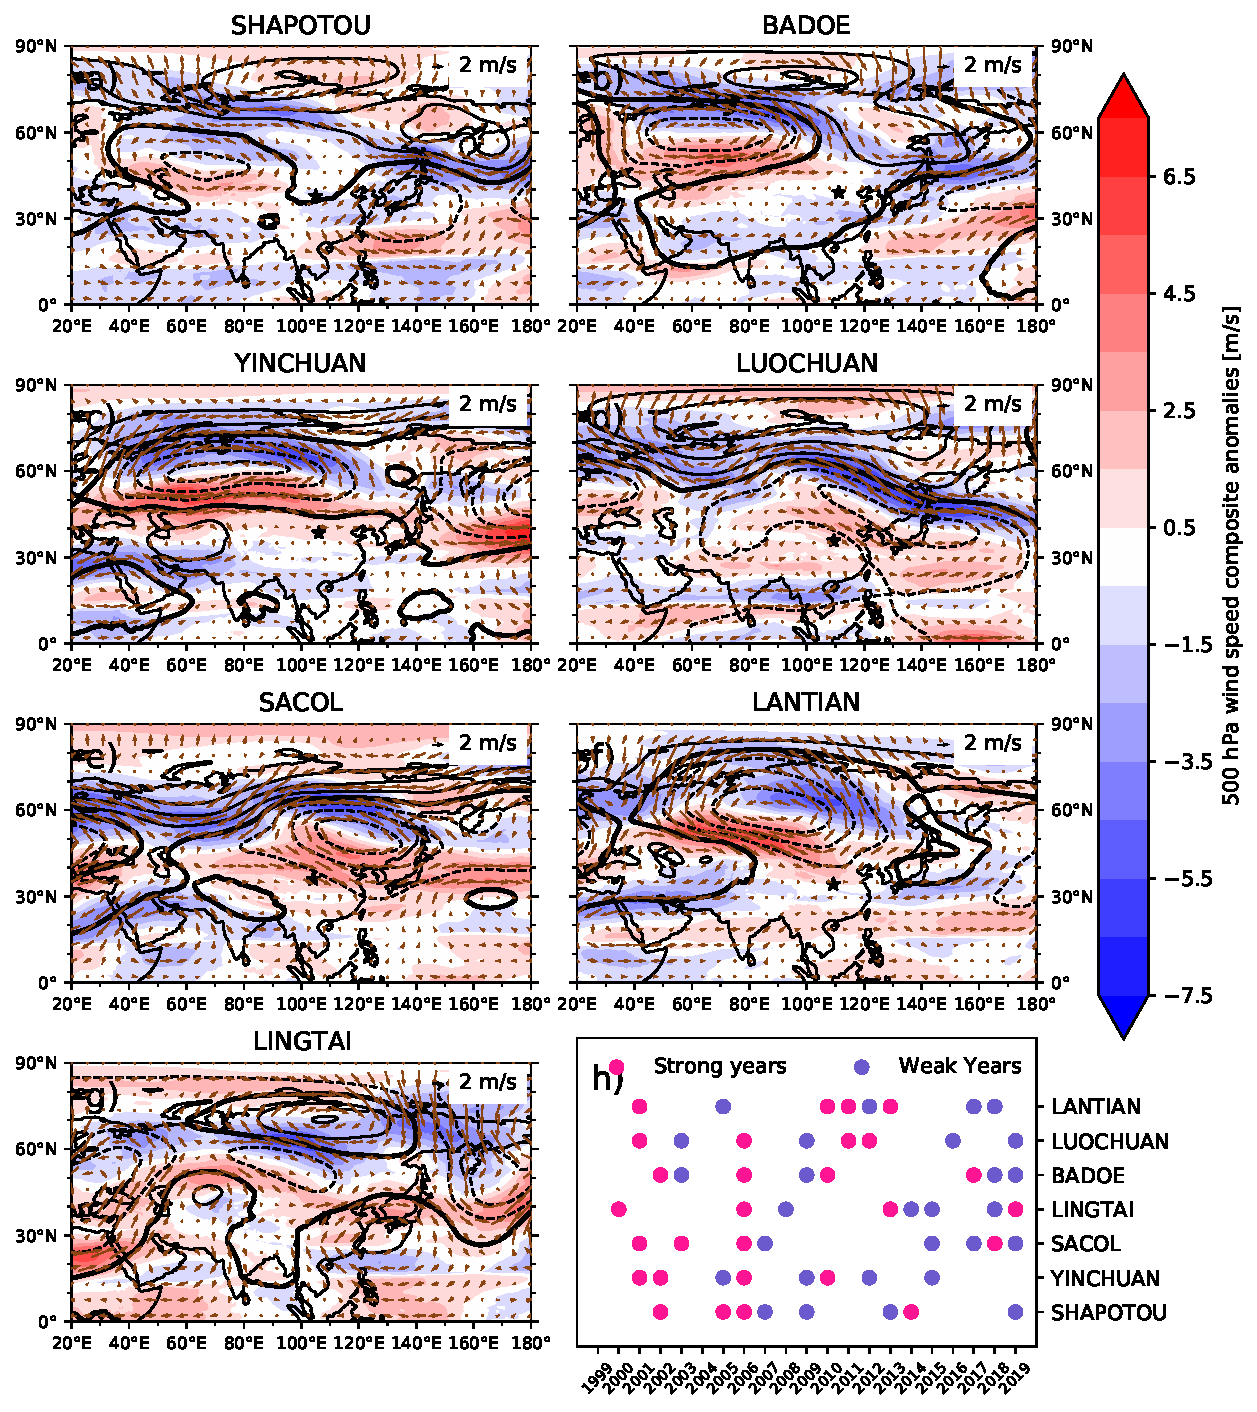
\includegraphics[width=\columnwidth]{texfiles/figs/20micrion_DJF_ws_geopot_500hPa.pdf}
    \caption{Composite difference anomalies of 500hPa geopotential height (contours) and 500hPa windspeed (shading) strong minus weak deposition years of the coarse size bin in winter (DJF) for all the locations a-g  (h) indicates which years are strong years and which years are weak.}
    \label{fig:DJF_500hPa_coarse_composite}
\end{figure}

\begin{figure}[hptb]
    \centering
    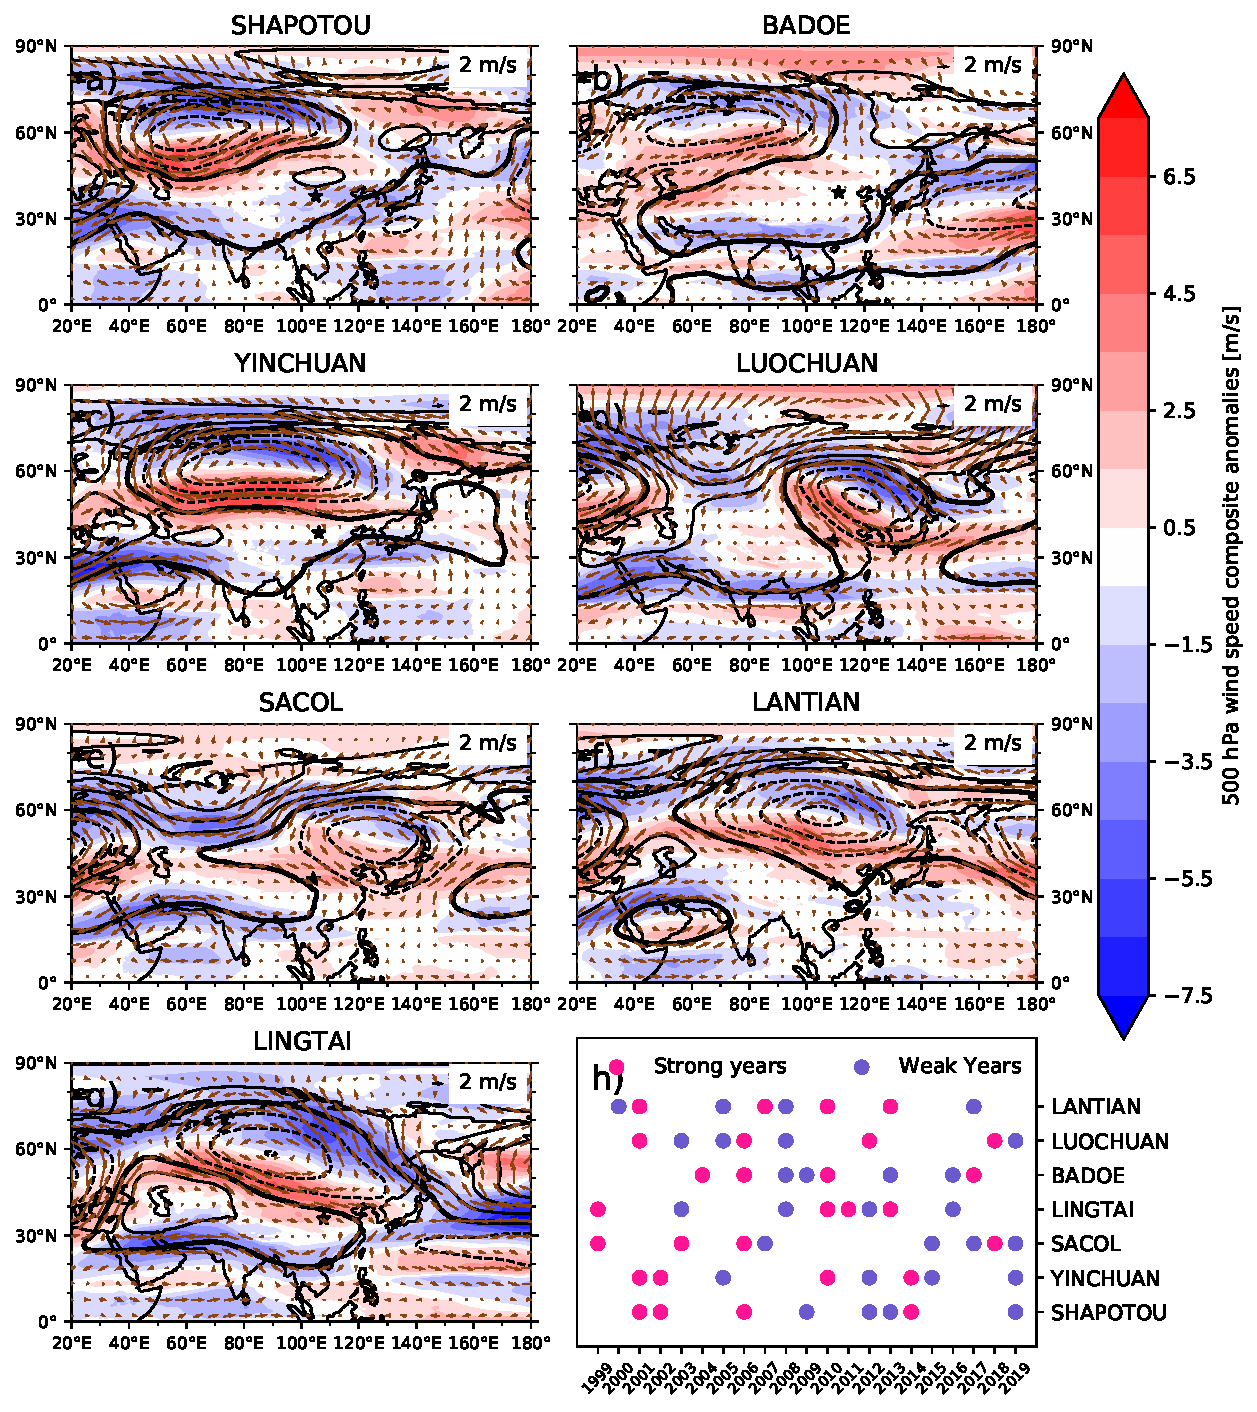
\includegraphics[width=\columnwidth]{texfiles/figs/2micrion_DJF_ws_geopot_500hPa.pdf}
    \caption{Composite difference anomalies of 500hPa geopotential height (contours) and 500hPa windspeed (shading) strong minus weak deposition years of the fine size bin in winter (DJF) for all the locations a-g  (h) indicates which years are strong years and which years are weak.}
    \label{fig:DJF_500hPa_fine_composite}
\end{figure}

